\documentclass{article}
\usepackage[UTF8, scheme = plain, zihao = 5, linespread = 1.3]{ctex}
\usepackage{indentfirst}
\usepackage{setspace, footmisc, hyperref, enumitem, fancyvrb, tikz}
\usepackage{mdframed, multicol, amsmath, bm, forest, hologo, manfnt}
\usepackage[a4paper, margin = 2.5cm]{geometry}
\usepackage[titles]{tocloft}
\usepackage[
	backend = biber, style = caspervector, utf8, giveninits = true
]{biblatex}
\usetikzlibrary{calc, math, positioning}
\addbibresource{up2020.bib}
\newcommand*{\docversion}{0.1.3}

\pagestyle{plain}
\setlength{\hfuzz}{3pt}
\setlength{\cftsecnumwidth}{2em}
\setlist{nolistsep, leftmargin = 3em}
\renewcommand{\thesection}{\ifnum\value{section}<10 0\fi\arabic{section}}
\renewcommand{\footnotelayout}{\ }
\renewcommand*{\bibfont}{\small}
\appto{\bibsetup}{\setlength{\hfuzz}{6pt}}
\newcommand*{\cmc}{black!81}
\newcommand*{\cmm}{\color{\cmc}\rmfamily\itshape}
\newcommand*{\cm}[1]{\cmm{#1}}
\tikzset{x = 1pt, y = 1pt}
\newcommand*{\tikzbase}{\tikzmath{
	\unity = \baselineskip; \unitx = 1.02 * \unity;
	\distx = 0.9em; \disty = 0.64em;
}}
\newcommand*{\tikzproc}[3]{\node at (#1 * \unitx - \distx, -#2 * \unity)
	[anchor = west] {\texttt{#3}}}
\newcommand*{\tikzcomment}[3]{\node at (#1, -#2 * \unity)
	[anchor = west] {\cm{#3}}}
\newcommand*{\tikzvline}[2]{
	\draw (#1 * \unitx, {-\disty - (#2 - 1) * \unity})
		-- (#1 * \unitx, -#2 * \unity)
}
\newcommand*{\tikzhline}[2]{
	\draw (#1 * \unitx, -#2 * \unity)
		-- ({(#1 + 1) * \unitx - \distx}, -#2 * \unity)
}

\newcommand{\specialsec}[1]{%
	\section*{#1}\addcontentsline{toc}{section}{#1}%
	\markboth{#1}{}\phantomsection%
}
\newcommand{\newpartx}[1]{%
	\addtocontents{toc}{\protect\vspace{#1\protect\baselineskip}}
	\clearpage%
}
\newcommand{\newpart}{\newpartx{1}}
\newcommand*{\stress}[1]{\textbf{#1}}
\newcommand*{\cupercite}[1]{\supercite{#1}\mbox{}}
\newcommand*{\colskipc}{\vspace{-0.25\baselineskip}}
\newcommand*{\bs}{\char92}
\RecustomVerbatimEnvironment{Verbatim}{Verbatim}%
	{baselinestretch = 1.2, formatcom = {\ifXeTeX\xeCJKVerbAddon\fi}}
\mdfdefinestyle{leftbar}{
	rightline = false, topline = false, bottomline = false,
	leftmargin = 2.45em, innerleftmargin = 0.65em,
	rightmargin = 3em, innerrightmargin = 0pt,
	innertopmargin = 0.36em, innerbottommargin = 0.3em,
	skipabove = {0.36\baselineskip}, skipbelow = {0.1\baselineskip}
}
\newmdenv[style = leftbar]{quoting}
\newmdenv[style = leftbar, rightmargin = 0pt]{wquoting}

\makeatletter
\newbibmacro*{eid+url+urldate}{%
	\printfield{eid}\setunit*{\bbx@cecomma}%
	\printfield{url}\setunit*{\bbx@cecomma}%
	\iffieldundef{urlyear}{}{%
		\printtext{\bbx@cetext{\bbx@cnretr}{accessed on}\addspace}%
		\iffieldundef{verba}{\printurldate}%
			{\href{\thefield{verba}}{\printurldate}}%
	}%
}
\makeatother


\newcommand*{\cf}{\emph{cf.}}
\newcommand*{\eg}{\emph{eg.}}
\newcommand*{\vs}{\emph{vs.}}
\newcommand*{\etc}{\emph{etc}}
\newcommand*{\etal}{\emph{et al}}
\newcommand*{\rnrs}[1]{\emph{R$^{#1}\!$RS}}
\newcommand*{\colskipa}{\vspace{-0.5\baselineskip}}
\newcommand*{\colskipb}{\vspace{-0.5\baselineskip}}

\begin{document}
\title{\textbf{Unix Philosophy 2020}}
\author{%
	Casper Ti.\ Vector
	\texttt{<\url{CasperVector@gmail.com}>}\\
	\url{https://gitea.com/CasperVector/up2020}%
}
\date{2019-08/2019-09; version \docversion}
\maketitle
\vspace{\baselineskip}
\tableofcontents

\newpartx{0.5}
\specialsec{Foreword}

I began learning Linux in the end of 2008, and using it in the beginning
of 2009; I have always used Linux as my main operating system thereafter.
During the course of using Linux and interacting with the ecosystem of
Unix-like operating systems, I got attracted to the notion of Unix
philosophy, and have benefited enormously from it.  (For more details on
the origin of this document, see the \hyperref[sec:afterword]{Afterword}.)
This document is a compendium of my thoughts about the Unix philosophy,
organised into three main parts, as are summarised below.

In the first part, we will first discuss the question ``\stress{what is the
essence of the Unix philosophy}?'', and I will argue that it is the minimisation
of the cognitive complexity of the system while almost satisfying the
requirements.  These years, many people think the philosophy, which originated
from legacy limitations on computational resources back in the 1970s, is no
longer applicable in software development.  So \stress{is the Unix philosophy
still relevant}, and will it still be relevant in the 2020s?  My answer is
``yes, and more relevant than when it was born''.  As a conclusion to this part,
I will give my experience about \stress{how the Unix philosophy can be followed
in actual use and development}, to the advantage of the user~/ developer.

In the second part, we will move our focus out of the field of programming, and
explore \stress{the applicability of the Unix philosophy in science, technology
and society, and the limits to that applicability}.  After the discussion on
science and technology, I will consider minimalism in philosophy, literature
and arts, and attempt to find a cognitive basis for minimalism and its limits;
the theory on the cognitive limits to minimalism will then be used to explain
why society often does not work like Unix.  As a conclusion, we will discuss
\stress{how minimalism can be adhered to, especially by the ordinary person},
to boost one's efficiency in everyday work.

In the third part, we will return to programming, but this time we will begin
with a digression about Lisp and especially Scheme, which also encourage
minimalism.  In order to understand the minimalism of Lisp, we will examine
the notion of homoiconicity, which I find as important as complexity.  I will
then try to answer ``\stress{what is the root of the antagonism between
Unix and Lisp}?'', and finally explore the benefits and feasibility of
\stress{a minimalist language framework which adopts the best
from Lisp and C}, and which also avoids the weaknesses.

Before actually diving into the main parts, it should be noted that this
document is meant to be read critically, for two reasons.  First, what I write
here is just my personal opinions about the Unix philosophy, and the latter
is just one way, among the many ones, to model the world.  Second, I still
know little about unfamiliar research fields like philosophy, cognitive
science, and programming languages, so the contents about these topics are
highly tentative, and there may well be points that turn out to be amateurish
or even ludicrous.  I attempted to avoid making mistakes in this document,
and please feel free to tell me if you find any.

This document is an extended transcript of my technical report,
\emph{Unix philosophy in the contemporary era}\cupercite{casper2018}, on
10 November 2018 for the Linux Club of Peking University; I consider it
as the culmination of my 10-year experience in the open-source community,
and dedicate it to the 50th anniversary of Unix\cupercite{salus2005}.
I enjoyed making the report as well as this document, and wish you
could also have some fun reading through the document, whether you
are a newcomer to the community, or an expert almost 3 times my age.

\newpage
\specialsec{How to read this document}

Due to feedback from multiple readers, it has been brought to my attention that
the nature of this document as a compendium -- a collection of thoughts about
various subjects -- can lead to some confusions: who are expected to read this
document, and how should they read the document?  Here I will briefly explain
the logical relation between the parts~/ sections in this document, and then
attempt to give a guide to readers with various backgrounds; please feel free
to tell me if you have any advice on how to make this document more accessible.

\begin{wquoting}
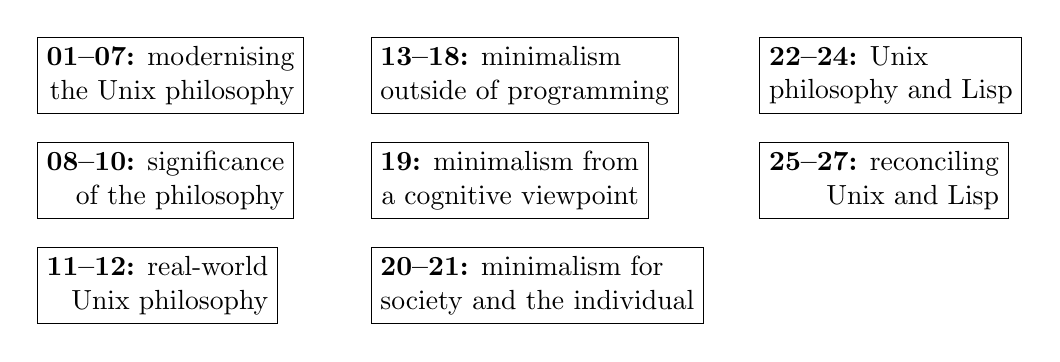
\begin{tikzpicture}[
	every node/.style = {draw, rectangle, font = \linespread{1}\selectfont},
	every matrix/.style = {
		draw = none, anchor = west, row sep = 1em, column sep = 2em
	}, ll/.style = {align = left}, rr/.style = {align = right}
]
	\newcommand*{\subj}[4]{\node [#1] {\textbf{#2:} #3\\#4}}
	\matrix {
		\subj{rr}{01--07}{modernising}{the Unix philosophy}; &[0.4em]
		\subj{ll}{13--18}{minimalism}{outside of programming}; &
		\subj{ll}{22--24}{Unix}{philosophy and Lisp}; \\
		\subj{rr}{08--10}{significance}{of the philosophy}; &
		\subj{rr}{19}{minimalism from}{a cognitive viewpoint}; &
		\subj{rr}{25--27}{reconciling}{Unix and Lisp}; \\
		\subj{rr}{11--12}{real-world}{Unix philosophy}; &
		\subj{ll}{20--21}{minimalism for}{society and the individual}; \\
	};
\end{tikzpicture}
\end{wquoting}

Above is an outline of the logical organisation of this document.  In my
opinion, nowadays the Unix philosophy is often neglected, questioned or
even distorted, due to misunderstanding about it.  So in the first part,
I will first present my attempt at a modernised formulation of the
philosophy in Sections~\ref{sec:intro}--\ref{sec:complex}.  Using the
formulation as the theoretical foundation, I will discuss significance
of the Unix philosophy in the contemporary context in Sections~%
\ref{sec:quality}--\ref{sec:foss}, and real-world applications
of the philosophy in Sections~\ref{sec:devel}--\ref{sec:user}.

I disagree with some people's opinion that the Unix philosophy was now
merely an aesthetic, because I believe it is rooted in human recognition,
which results in its inherent importance.  In the second part, using the
above-mentioned formulation, I will first examine some analogues to the Unix
philosophy outside of the field of programming in Sections~\ref{sec:hilbert}%
--\ref{sec:art}.  After that, I will present my cognitive justification
for the philosophy in Section~\ref{sec:cognitive}, and discuss its
value for society and the individual in Sections~\ref{sec:society}--%
\ref{sec:worklife}, similar to the last two sections in the first part.

In the recent years, it has gradually become my opinion that expertise from
the Unix and Lisp circles can be joined to build systems that are more
Unix-ish than was possible before.  So in the third part, I will first
discuss the relation between Lisp and the previously formulated Unix
philosophy in Sections~\ref{sec:lisp}--\ref{sec:wib}.  Finally, I will
examine the benefits of the proposed Unix~/ Lisp reconciliation, and how this
reconciliation can be achieved in Sections~\ref{sec:benefits}--\ref{sec:toe}.

It is generally recommended to read this document in the original order, and
just skip parts~/ sections you are less interested in; however, Section~%
\ref{sec:complex} lays the theoretical foundation for this document, so you
should at least skim through it.  Quite a few examples from the ``init war''
are used in the first part, so people entangled in related events are advised
to read that part.  Those who like philosophical discussions might feel
interested in the second part.  Unix developers interested in programming
languages, as well as researchers of these languages, will perhaps find
the third part attractive.  Footnotes are generally less essential
contents, and often require deeper understanding of the subject matter.

\newpart
\section{An introduction to the history of Unix}\label{sec:intro}

CTSS\cupercite{wiki:ctss} (first released in 1961), widely thought to be the
first time-sharing operating system in history, was quite a success; its success
resulted in a much more ambitious project called Multics\cupercite{wiki:multics}
(with development starting in 1964), which did not deliver a commercially usable
system until 1969\cupercite{multicians:history} despite joint efforts from
MIT, GE and Bell Labs, as the system was too complicated for the human and
computational resources available at that time\footnote{\label{fn:multics}%
Actually, what the system required is no more than the hardware of a low-end
home router now, and in comparison, modern Linux systems can only run on the
same hardware with massive tailorings to reduce the size.  The Multicians
Website has a page\cupercite{multicians:myths} clarifying some common
misunderstandings about Multics.}.  Bell Labs withdrew from the project in 1969,
a few months before the first commercial release of Multics; Ken Thompson and
Dennis Ritchie, previosuly working on the project, went on to develop another
operating system to fulfill their own needs, and the system would soon get the
name ``Unix''\cupercite{wiki:unixhist}.  In order to make the new system usable
and manageable on a (sort of) spare PDP-7 minicomputer at Bell Labs, Thompson
made major simplifications to the Multics design and only adopted certain key
elements like the hierarchical file system and the shell\cupercite{seibel2009}.

The 1970s saw the growth and spread of Unix (\cf~\parencite{wiki:unixhist}
for the details), and in my opinion the most important historical event
during this period was the publication of \emph{Lions' Commentary on Unix
v6}\cupercite{wiki:lions}\footnote{For a modern port of Unix v6, \cf~%
\parencite{wiki:xv6}.} in 1976, which greatly spurred the propagation of Unix
in universities.  In the early 1980s, commercial versions of Unix by multiple
vendors appeared, but AT\&T, the owner of Bell Labs at that time, was barred
from commercialising Unix due to antitrust restrictions; this changed in
1983, when the Bell System was broken up, and AT\&T quickly commercialised
Unix and restricted the distribution of its source code.  The restriction on
code exchange greatly contributed to the already looming fragmentation of Unix,
resulting in what we now call the ``Unix wars''\cupercite{raymond2003a}; the
wars, in combination with the negligence of 80x86 PCs' potentials by the Unix
circle, led to the pitiful decline in popularity of Unix in the 1990s.

In 1991, Linus Torvalds started working on his own operating system kernel,
which went on to become Linux; the combination of userspace tools from the
GNU project (starting from 1985) and the Linux kernel achieved the goal of
providing a self-hosting Unix-like environment that is free / open-source and
low-cost\footnote{The 386BSD project also reached this goal, but its first
release was in 1992; additionally, a lawsuit and some infighting at that
time\cupercite{wiki:386bsd} distracted the BSD people, and now it might be
fair to say that, from then on, BSD never caught up with Linux in popularity.},
and kickstarted the GNU/Linux ecosystem, which is perhaps the most important
frontier in the open-source movement.  Currently, the most popular Unix-like
systems are undisputedly Linux and BSD, while commercial systems like Solaris
and QNX have minute market shares; an unpopular but important system,
which I will introduce in Section~\ref{sec:plan9}, is Plan~9
from Bell Labs (first released in 1992).

Before ending this section which has hitherto been mostly non-technical,
I would like to emphasise the three techical considerations which
``influenced the design of Unix'' according to Thompson and Ritchie
themselves\cupercite{ritchie1974}, and all of these points
will be discussed in later sections:
\begin{itemize}
\item \stress{Friendliness to programmers}: Unix was designed to boost
	the productivity of the user as a programmer; on the other hand,
	we will also discuss the value of the Unix methodology from
	a user's perspective in Section~\ref{sec:user}.
\item \stress{Simplicity}: the hardware limitations on machines accessible
	at Bell Labs around 1970 resulted in the pursuit of economy and elegance
	in Unix; as the limitations are no more, is simplicity now only an
	aesthetic?  Let's see in Sections~\ref{sec:quality}--\ref{sec:foss}.
\item \stress{Self-hosting}: even the earliest Unix systems were able to be
	maintained independent of machines running other systems; this requires
	self-bootstrapping, and its implications will be discussed in Sections~%
	\ref{sec:security}~\& \ref{sec:benefits}--\ref{sec:howto}.
\end{itemize}

\section{A taste of shell scripting}\label{sec:shell}

It was mentioned in last section that the shell was among the few design
elements borrowed by Unix from Multics; in fact, as the main way that the user
interacts with the system\cupercite{ritchie1974} (apart from the graphical
interface), the shell is also a component where the design concepts of Unix
are best reflected.  As an example, we can consider the classic word frequency
sorting problem\cupercite{robbins2005} -- write a program to output the $n$
most frequent words along with their frequencies; this problem attracted
answers from Donald Knuth, Doug McIlroy and David Hanson.  The programs by
Knuth and Hanson were respectively written from scratch in Pascal and C, and
each took a few hours to write and debug; the program by McIlroy was a shell
script, which took only one or two minutes and worked correctly on the
first run.  This script, with minor modifications, is shown below:
\begin{quoting}
\begin{Verbatim}
#!/bin/sh
tr -cs A-Za-z\' '\n' | tr A-Z a-z |
sort | uniq -c |
sort -k1,1nr -k2 | sed "${1:-25}"q
\end{Verbatim}
\end{quoting}

Its first line tells Unix this is a program interpreted by \verb|/bin/sh|,
and the commands on the rest lines are separated by the
\stress{pipe} ``\verb/|/'' into six steps:
\begin{itemize}
\item In the first step, the \verb|tr| command converts all
	characters, except for (uppercase and lowercase) English
	letters and ``\verb|'|'' (the \verb|-c| option means to complement),
	into the newline character \verb|\n|, and the \verb|-s| option
	means to squeeze multiple newlines into only one.
\item In the second step, the command converts all uppercase letters into
	corresponding lowercase letters; after this step, the input text is
	transformed into a form where each line contains a lowercase word.
\item In the third step, the \verb|sort| command sorts the lines according
	to the dictionary order, so that the same words would appear on
	adjacent output lines.
\item In the fourth step, the \verb|uniq| command replaces repeating adjacent
	lines with only one of them, and with the \verb|-c| option prepends to the
	line the count of the repetition, which is also the frequency we want.
\item In the fifth step, the \verb|sort| command sorts the lines according to
	the first field (the frequency added in last step) in descending numerical
	order (the \verb|-k1,1nr| option, where \verb|n| defaults to the
	ascending order, and \verb|r| reverses the order), and according
	to the second field (the word itself, with the \verb|-k2| option)
	in dictionary order in case of identical frequencies.
\item In the sixth step, the \verb|sed| command only prints the first lines,
	with the actual number of lines specified by the first argument of the
	script on its execution, defaulting to 25 when the argument is empty.
\end{itemize}
Apart from being easy to write and debug, this script is also very maintainable
(and therefore very customisable), because the input requirements and processing
rules of the steps are very simple and clear, and we can easily replace the
actual implementations of the steps: for instance, the word-splitting criterion
used above is obviously primitive, with no consideration of issues like
stemming (\eg~regarding ``look'', ``looking'' and ``looked'' as the
same word); if such requirements are to be implemented, we only need
to replace the first two steps with some other word-splitting program
(which probably needs to be written separately), and somehow make
it use the same interface as before for input and output.

Like many Unix tools (\eg~the ones used above), this script reads input from
its \stress{standard input} (defaults to the keyboard), and writes output to
its \stress{standard output} (defaults to the current terminal)\footnote{The
\texttt{stdio.h} in C means standard I/O exactly.}.  Input/output from/to a
specified file can be implemented with the \stress{I/O redirection} mechanism
in Unix, for example the following command in the shell (assuming the script
above has the name \verb|wf.sh| and has been granted execution permission)
\begin{quoting}
\begin{Verbatim}
/path/to/wf.sh 10 < input.txt > output.txt
\end{Verbatim}
\end{quoting}
outputs the 10 most frequent words, with their frequencies, from
\verb|input.txt| into \verb|output.txt|.  It is obvious that the pipe is also
a redirection mechanism, which redirects the output of the command on its
left-hand side to the input of the command on its right-hand side.  From another
perspective, if the commands connected by pipes are considered as filters, then
each filter performs a relatively simple task, and the programming style in the
script above is to decompose a complicated text-processing task into multiple
filtering steps linked together with pipes, and then to implement the steps
with relatively ready-made tools.  Through the example above, we have taken a
glimpse at the strong power that can be achieved by the combination of Unix
tools; but other systems, like Windows, also have mechanisms similar to I/O
redirection, pipes \etc{} in Unix, so why don't we often see similar
usage in these systems?  Please read the next section.

\section{Cohesion and coupling in software engineering}\label{sec:coupling}

Cohesion and coupling are extremely important notions in software engineering,
and here we first try to understand what coupling is.  Consider the interactions
(\eg~communication through text or binary byte streams, message passing using
data packets or other media, calls between subroutines) between modules in
the two extreme cases from the figure in \parencite{litt2014a}.  When some
faults occur, how difficult will the debugging processes be with the two
systems?  When the requirements change, how difficult will the maintenance be
with the two systems?  I think the answer should be self-evident.  In these two
systems, similarly consisting of 16 modules, the sharp difference in the level
of difficulty in debugging and maintenance is determined by the complexity
of interactions between modules, and the \stress{degree of coupling} can just
be considered as a measure of the complexity of this kind of interactions.
We obviously want the modules in a system to be as loosely coupled as
reasonable, and the script from last section was easily to debug and
maintain exactly because of the low coupling between the underlying commands.

Low coupling is actually a common feature of traditional Unix tools, so why can
they be loosely coupled?  A tip of the iceberg has already been shown in the
script from the last section: the tools not only have well-defined input/output
interfaces, but also have clear processing rules from the input to the output,
or in other words their behaviours are clearly guided; from the perspective of
systems and modules, each Unix tool, when considered as a module, usually does
a different unit operation, like character translation (\verb|tr|), sorting
(\verb|sort|), deduplication / counting (\verb|uniq|) and so on.  When Unix
tools are implemented, each of them usually also needs to be partitioned into
submodules, but the submodules are always much more tightly coupled than the
tools themselves are, even with a most optimal design; for this reason, when
partitioning a system into modules, it is desirable to concentrate this kind
of coupling inside the modules, instead of exposing them between the modules.
I consider the \stress{degree of cohesion} to be the measure of this
kind of inherent coupling between submodules inside a module, and
partitioning of a system according to the principle of high cohesion
would naturally enforce clear separation of concerns between modules,
and therefore reduce the degree of coupling in the system.

We have already seen that high cohesion and low coupling are desirable
properties for software systems.  You might ask, while there are many Windows
programs that are loosely coupled (\eg~Notepad and Microsoft Paint do not
depend upon each other) and have somehow high cohesion (\eg~Notepad is used
for text editing while Microsoft Paint for drawing), why don't we often combine
them as with Unix tools?  The answer is actually obvious -- because they are
not designed to be composable; to put it more explicitly, they cannot use some
simple yet general-purpose interface, like pipes, to collaborate, and therefore
cannot be easily reused in automated tasks.  In comparison, the power of
Unix seen in last section comes exactly from its emphasis on reusability of
user-accessible tools in automation, which results in the almost extreme
realisation of the principle of high cohesion and low coupling in traditional
Unix tools\cupercite{salus1994}.  In conclusion, the requirements of cohesion
and coupling must be considered with the background of \stress{collaboration
and reuse}, and the pursuit of collaboration and reuse naturally
promotes designs with high cohesion and low coupling.

Until now, our examples have been relatively idealised or simplified, and here
I give two more examples that are more realistic and relevant to hot topics in
recent years.  When Unix systems are started, the kernel will creates a first
process, which in turn creates some other processes, and these processes manage
the system services together; because of the important role of the first process
in system initialisation, it is usually called ``\stress{init}''\cupercite%
{jdebp2015}.  systemd is the most popular init system as of now, and its init
has very complex functionalities, while its mechanisms are poorly documented;
furthermore, aside from the init program called \verb|systemd| as well as
related ancillary programs, systemd also has many other non-init modules, and
the interactions between all these modules are complex and lack documentation
(a fairly exaggerated depiction can be found at \parencite{litt2014b}).
systemd obviously has low cohesion and high coupling, but this is unnecessary
because the daemontools-ish design (represented in this document with s6) is
much simpler than systemd, yet not weaker than systemd in functionalities.

The init program of s6, \verb|s6-svscan|, scans for subdirectories in a
specified directory (``scan directory'', like \verb|/service|), and for each
subdirectory (``service directory'', like \verb|/service/kmsg|) runs a
\verb|s6-supervise| process, which in turn runs the executable called \verb|run|
in the scan directory in order to run the corresponding system service.
The user can use s6's command line tools \verb|s6-svc|/\verb|s6-svscanctl|
to interact with \verb|s6-supervise|/\verb|s6-svscan|, and can use ancillary
files in service directories and the scan directory to modify the behaviours
of \verb|s6-supervise| and \verb|s6-svscan|\footnote{This configuration method
may seem unintuitive, but its rationale and benefits will be explained in
Section~\ref{sec:homoiconic} and Footnote~\ref{fn:slew}.}.  Only longrun
services are managed by s6, while oneshot init scripts are managed by s6-rc,
which also uses s6's tools to track the startup status of services in order
to manage the dependency between them.  It was mentioned above that this
design is not weaker than systemd in functionalities, and here I give one
example (\cf~Section~\ref{sec:exec} for some in-depth examples): systemd
supports service templates, for instance after a template called \verb|getty@|
is defined, the \verb|getty@tty1| service would run the getty program on
\verb|tty1|; in s6/s6-rc, a similar functionality can be achieved by calling
a 5-line library script\cupercite{gitlab:srvrc} in the \verb|run| script.

\section{Do one thing and do it well}\label{sec:mcilroy}

The Unix-ish design principle is often called the ``\stress{Unix philosophy}'',
and the most popular formulation of the latter is undoubtedly
by Doug McIlroy\cupercite{salus1994}:
\begin{quoting}
	This is the Unix philosophy:  Write programs that do one thing and
	do it well.  Write programs to work together.  Write programs to
	handle text streams, because that is a universal interface.
\end{quoting}

In connection with the discussion in last section, it is easy to notice
that the first point by McIlroy is an emphasis on high cohesion and low
coupling\footnote{By the way, this also shows that the requirements of high
cohesion and low coupling is not unique to objected-oriented programming.
In fact, some people believe\cupercite{chenhao2013} that every design pattern
in OOP has some counterparts in Unix (\cf~Section~\ref{sec:exec} for one of
them).}, the second point is an emphasis on collaboration and reuse of
programs, and the third point feels slightly unfamiliar: we did see the power
from combination of Unix tools in text processing in Section~\ref{sec:shell},
but what is the underlying reason for calling text streams a universal
interface?  I believe that this can be explained by the friendliness of
\stress{human-computer interfaces} toward humans and computers (this will
be involved again in Section~\ref{sec:cognitive}), where text streams are a
compromise between binary data and graphical interfaces.  Binary data are easily
processed by computers, but are difficult to understand for humans, and the
subtle differences between the ways binary data are processed by different
processors also give rise to portability issues of encodings, with the
endianness problem being a representative issue.  Graphical interfaces are
the most friendly to humans, but are much more difficult to write in comparison
with textual interfaces, and do not compose easily even as of now\footnote{It is
worth mentioning that I do not reject graphical interfaces, but just think the
requirements of automation need consideration in their design; and as far
as I know, the automation of graphical interfaces is still a non-trivial
subject.  I currently find the AutoCAD design an interesting approach, where
there is a command line along with the graphical interface, and operations on
the graphical interface are automatically translated into commands and shown
on the command line.}.  Text streams are both easy for computers to process
and fairly easy for humans to understand, and while it also involves issues
with character encoding, the latter kind of issues are generally
much simpler than similar issues with binary information.

McIlroy's formulation is not undisputed, and the most relevant disagreement is
on whether text streams as a communication format is the best choice, which we
will also discuss in Section~\ref{sec:wib}; in addition, while this formulation
almost covers the factors that we have hitherto seen to make Unix powerful,
I do not think it completely represents the Unix philosophy.  It is worth
noting that the appearance of pipes directly resulted in the pursuit of
collaboration and reuse of command line programs\cupercite{salus1994}, and
McIlroy is the inventor of Unix pipes, so his summary was obviously based on
shell scripting.  Shell scripting is admittedly important, but it is far
from the entirety of Unix: in the two following sections, we will see
some relevant cases outside shell scripting that however reflect the
philosophy, which cannot be covered by the classic formulation by
McIlroy; and then in Section~\ref{sec:complex}, I will present
what I regard as the essence of the Unix philosophy.

\section{\texttt{fork()} and \texttt{exec()}}\label{sec:exec}

Processes are one of the most important notions in operating systems, so OS
interfaces for process management are quite relevant; as each process has a
set of state attributes, like the current working directory, handles to open
files (called \stress{file descriptors} in Unix, like the standard input and
output used in Section~\ref{sec:shell}, and the \stress{standard error output}
which will be involved in Section~\ref{sec:complex}) \etc, how do we create
processes in specified states?  In Windows, the creation of processes is
implemented by the \verb|CreateProcess()| family of functions, which usually
needs about 10 arguments, some of which are structures representing multiple
kinds of information, so we need to pass complicated state information when
creating processes; and noticing that we need system interfaces to modify
process states anyway, the code that does these modifications are nearly
duplicated in \verb|CreateProcess()|.  In Unix, processes are created using
the \verb|fork()| function, which initiates a new child process with state
attributes identical to the current process, and the child process can replace
itself with other programs by calling the \verb|exec()| family of functions;
before \verb|exec()|ing, the child process can modify its own state attributes,
which are preserved during \verb|exec()|.  It is obvious that \verb|fork()|/%
\verb|exec()| only require very little information, and that Unix realised the
decoupling between process creation and process state control through this
mechanism; and considering that when creating processes in real applications,
the child process often need to inherit most attributes from its parent,
\verb|fork()|/\verb|exec()| actually also simplifies the user code greatly.

If you know some object-oriented programming, you should be easily able to
notice that the \verb|fork()|/\verb|exec()| mechanism is exactly a realisation
of the Prototype Pattern, and the same line of thought can also inspire us
to think about the way processes are created for system services.  With systemd,
service processes are created by its init program \verb|systemd|, which reads
configuration file(s) for each service, runs the corresponding service program,
and sets the process attributes for the service process according to the
configuration; under this design, all the code for process creation and process
state control need to be in the init, or in other words what systemd does is
like, on a conceptual sense, implementing service process creation in the style
of \verb|CreateProcess()| while using \verb|fork()|/\verb|exec()|.  Borrowing
the previous line of thought, we can completely decouple process state control
from the init module: for example, with s6, \verb|s6-supervise| almost does
not modify any process attribute before \verb|exec()|ing into the \verb|run|
program; the \verb|run| program is almost always a script (\cf~\parencite%
{pollard2014} for some examples), which sets its own attributes before
\verb|exec()|ing into the actual service program.  The technique of implementing
process state control with consecutive \verb|exec()|s is expressively called
\stress{Bernstein chainloading}, because of Daniel J.\ Bernstein's extensive use
of this technique in his software qmail (first released in 1996) and daemontools
(first released in 2000); Laurent Bercot, the author of s6, pushed this
technique further and implemented the unit operations in chainloading as a set
of discrete tools\cupercite{ska:execline}, with which we can implement some very
interesting requirements (\cf~Footnote~\ref{fn:logtype} for one such example).

When creating service processes, chainloading is of course much more flexible
than systemd's mechanism, because the modules of the former possess the
excellent properties of high cohesion and low coupling, and are therefore easy
to debug and maintain; in comparison, the mechanism in systemd is tightly
coupled to other modules from the same version of systemd, so we cannot easily
replace the malfunctioning modules when problems (\eg~\parencite{edge2017})
arise.  Because of the simple, clear interface of chainloading, when new process
attributes emerge, we can easily implement the corresponding chainloader, and
then integrate it into the system without upgrading: for instance, systemd's
support for Linux's cgroups is often touted by systemd developers as one of its
major selling points\cupercite{poettering2013}, but the user interface is just
operations on the \verb|/sys/fs/cgroup| directory tree, which are easy to do in
chainloading; now we already have some ready-made chainloaders available%
\cupercite{pollard2019}, so it can be said that the daemontools-ish design has
natural advantages on support for cgroups.  Additionally, the composability of
chainloaders allow us to implement some operations that are hard to describe
just using systemd's mechanisms: for example we can first set some environment
variables to modify the behaviour of a later chainloader, and then clear the
environment before finally \verb|exec()|ing into the service program;
\cf~\parencite{ska:syslogd} for a more advanced example.

It is necessary to note that primitive forms of \verb|fork()|/\verb|exec()|
appeared in operating systems earlier than Unix\cupercite{ritchie1980}, and
Ken Thompson, Dennis Ritchie \etal{} chose to implement process creation with
this mechanism out of a pursuit of simplicity of the implementation, so the
mechanism was not exactly an original idea in Unix; nevertheless we have also
seen that based on \verb|fork()|/\verb|exec()| and its line of thought we can
implement many complicated tasks in simple, clear ways, so the mechanism does
satisfy the Unix design concepts in Section~\ref{sec:shell} in an intuitional
sense.  Now back to the subject of Unix philosophy: \verb|fork()|/\verb|exec()|
conforms to the principle of high cohesion and low coupling, and facilitates
collaboration and reuse of related interfaces, so we can regard it as roughly
compliant to the first two points from Doug McIlroy's summary in last
section despite the fact that it is not directly reflected in shell
scripting; however, this mechanism does not involve the choice of
textual interfaces, so it is not quite related to McIlroy's last point,
and I find this to be a sign that \verb|fork()|/\verb|exec()| cannot
be satisfactorily covered by McIlroy's formulation.

\section{From Unix to Plan~9}\label{sec:plan9}

Unix v7\cupercite{mcilroy1987} already had most notions seen currently
(\eg~files, pipes and environment variables) and many \stress{system
calls} (how the userspace requests services from the kernel, like
\verb|read()|/\verb|write()| which performs read/write operations on files,
and \verb|fork()|/\verb|exec()| mentioned in last section) that are still
widely used now.  To manipulate the special attributes of various hardware
devices and avoid a crazy growth in number of system calls with the development
of device support, this Unix version introduced the \verb|ioctl()| system call,
which is a ``jack of all trades'' that manipulates various device attributes
according to its arguments, for instance
\begin{quoting}
\begin{Verbatim}
ioctl (fd, TIOCGWINSZ, &winSize);
\end{Verbatim}
\end{quoting}
saves the window size of the serial terminal corresponding to the file
descriptor \verb|fd| into the structure \verb|winSize|.  In Unixes up to this
version (and even versions in few years to come), although there were different
kinds of system resources like files, pipes, hardware devices \etc{} to operate
on, these operations were generally implemented through file interfaces
(\eg~read/write operations on \verb|/dev/tty| are interpreted by the kernel
as operations on the terminal), or in other words ``everything is a file''; of
course, as was mentioned just now, in order to manipulate the special attributes
of hardware, an exception \verb|ioctl()| was made.  In comparison with today's
Unix-like operating systems, Unixes of that age had two fundamental differences:
they had no networking support, and no graphical interfaces; unfortunately,
the addition of these two functionalities drove Unix increasingly
further from the ``everything is a file'' design.

Berkeley sockets\cupercite{wiki:sockets} appeared in 1983 as the user interface
for the TCP/IP networking protocal stack in 4.2BSD, and became the most
mainstream interface to the internet in 1989 when the corresponding code was
put into the public domain by its copyright holder.  Coming with sockets was a
series of new system calls like \verb|send()|, \verb|recv()|, \verb|accept()|
\etal.  Sockets have forms similar to files, but they expose too many protocol
details, which make their operations much more complicated than those of files,
and a typical example for this can be seen at \parencite{pike2001}; moreover,
duplication began to appear between system calls, for example \verb|send()| is
similar to \verb|write()|, and \verb|getsockopt()|/\verb|setsockopt()| are
similar to the already ugly \verb|ioctl()|.  After that, the system calls began
to grow constantly: for instance, Linux currently has more than 400 system
calls\cupercite{kernel:syscalls}, while Unix v7 had only about 50\cupercite%
{wiki:unixv7}; one direct consequence of this growth is the complication of
the system interfaces as a whole, and the weakening of their uniformity, which
led to an increase in difficulty of learning.  The X Window System\cupercite%
{wiki:xwindow} (usually called ``X'' or ``X11'' now), born in 1984, has
problems similar to those of Berkeley sockets, and the problems are more
severe: sockets are at least formally similar to files, while windows
and other resources in X are not files at all; furthermore, although
X did not introduce new system calls as with sockets, its number
of basic operations, which can be roughly compared to system calls,
is much larger than the number of system calls related to sockets,
even when we only count the core modules of X without any extension.

After the analysis above, we would naturally wonder, how can we implement the
support for networking and graphical interfaces in Unix, in a way that follows
its design principles?  Plan~9 from Bell Labs (often simply called ``Plan~9'')
is, to a large extent, the product of the exploration on this subject by Unix
pioneers\cupercite{raymond2003b}.  As was mentioned before, system calls like
\verb|ioctl()| and \verb|setsockopt()| were born to handle operations on
special attrbutes of system resources, which do not easily map to operations
on the file system; but on a different perspective, operations on resource
attributes are also done through communication between the userspace and the
kernel, and the only difference is that the information passed in the
communication is special data that represent operations on resource attributes.
Following this idea, Plan~9 extensively employs \stress{virtual file systems}
to represent various system resources (\eg~the network is represented by
\verb|/net|), in compliance with the ``everything is a file'' design%
\cupercite{pike1995}; control files (\eg~\verb|/net/tcp/0/ctl|) corresponding
to various resource files (\eg~\verb|/net/tcp/0/data|) implement operations
on resource attributes, different \stress{file servers} map file operations
to various resource operations, and the traditional \stress{mounting}
operation binds directory trees to file servers.  Because file servers use
the network-transparent \stress{9P protocol} to communicate, Plan~9 is
naturally a distributed OS; in order to implement the relative independence
between processes and between machines, each process in Plan~9 has its own
\stress{namespace} (\eg~a pair of parent and child processes can see mutually
independent \verb|/env|, this way the independence of environment variables
is implemented), so normal users can also perform mounting.

With the mechanisms mentioned above, we can perform many complicated tasks in
Plan~9 in extremely easy ways using its roughly 50 system calls\cupercite%
{aiju:9syscalls}: for instance, remote debugging can be done by mounting
\verb|/proc| from the remote system, and the requirements of VPN can be
implemented by mounting a remote \verb|/net|; another example is that the
modification of users' networking permissions can be performed by setting
permissions on \verb|/net|, and that the restriction of user access to one's
graphical interface can be done by setting permissions on \verb|/dev/mouse|,
\verb|/dev/window| \etc.  Again back to the topic of Unix philosophy: on an
intuitional level, the design of Plan~9 is indeed compliant to the philosophy,
but even if \verb|fork()|/\verb|exec()|, analysed in last section, could be
said to be roughly compliant to Doug McIlroy's formulation on the philosophy
in Section~\ref{sec:mcilroy}, I am afraid that the ``everything is a file''
design principle can hardly be covered by the same formulation; so
the formulation was not very complete, and we need a better one.

\section{Unix philosophy: minimising the system's complexity}\label{sec:complex}

In the two previous sections, we have already seen that Doug McIlroy's
summary cannot satisfactorily cover the entirety of Unix philosophy;
this summary (and especially its first point) can indeed be regarded as
the most mainstream one, but there are also many summaries other than
the one by McIlroy\cupercite{wiki:unixphilo}:
\begin{itemize}
\item Brian Kernighan and Rob Pike emphasised the design of software systems as
	multiple easily composable tools, each of which does one kind of simple
	tasks in relative separation, and they in combination can do complex tasks.
\item Mike Gancarz\footnote{He is, curiously, one of the designers of the
	X Window System (\cf~Section~\ref{sec:plan9}).} summarised
	the Unix philosophy as 9 rules.
\item Eric S.\ Raymond gave 17 rules in \emph{The Art of Unix Programming}.
\end{itemize}
I believe that the various formulations of the philosophy are all of some value
as references, but they themselves also need to be summarised, just like how
Plan~9, as was mentioned in last section, implemented requirements, which need
several hundreds of system calls elsewhere, with only about 50 system calls
by using virtual file systems, the 9P protocol and namespaces.  In Sections~%
\ref{sec:shell}~\& \ref{sec:exec}--\ref{sec:plan9}, our intuitive criteria
for a system's conformance to the Unix philosophy were all that the system
used a small number of simple mechanisms and tools to implement requirements
that were more difficult to implement in other ways, or in other words they
reduced the complexity of the system.  Based on this observation, I believe
the essence of the Unix philosophy is \stress{the minimisation of the cognitive
complexity of the system while almost satisfying the requirements}\footnote%
{Some people noted that while this formulation can be used to compare existing
software systems and practical plans for such systems, it does not directly
tell us how to design and implement minimal software systems.  However, the
formulation does cover existing summaries for the Unix philosophy, which
are more practical; it also indirectly leads to the practical ways to foster
minimalist habits (and creativity) in Sections~\ref{sec:devel}--\ref{sec:user}.
I regard the relation between this formulation and practical ways to minimal
software systems as similar to the relation between the principle of least
action and the calculus of variations, as well as to the relation between
the Ockham's razor and the theories about the minimal message length
and the minimal description length (\cf~Section~\ref{sec:ockham}).},
and the three restrictions in my formulation are explained below:
\begin{itemize}
\item The prerequisite is to \stress{almost} satisfy the requirements,
	because said requirements can often be classified into core parts
	(\eg~support for networking and graphical interfaces) and non-core
	parts (\eg~support for Berkeley sockets and the X Window System),
	and some non-core parts can be discarded or implemented in better ways.
\item We need to consider the total complexity of the \stress{system}, because
	there are interactions between the modules, and only examining some of the
	modules would result in omission of the effects on their behaviours by
	their dependencies: for example, if a requirement could be implemented in	
	both ways in the figure from \parencite{litt2014a}, and both implementations
	use the same user interface, we surely cannot say they would be equally
	compliant to the Unix philosophy just because of the identical interfaces.
\item It is stipulated that we are discussing about the \stress{cognitive}
	complexity, because as was shown in the comparison above (a more realistic
	comparison can be found at \parencite{github:acmetiny}/\parencite%
	{gitlab:emca}), the quality of a system is not only determined by its code
	size; we also have to consider the cohesion and coupling of its modules,
	and the latter are essentially attributes oriented toward humans, not
	computers, which I will further discuss in Section~\ref{sec:cognitive}.
\end{itemize}

Let's see a fairly recent example.  In some init systems (represented by
sysvinit), longrun system services detach themselves from the control of the
user's shell, in order to implement backgrounding\cupercite{gollatoka2011}:
when the service program is run by the user from the shell, it \verb|fork()|s a
child process, and then the parent process exits, so the shell waits for another
command from the user because the user-run (parent) process has exited, while
the child process is reparented to init upon exiting of the parent process, and
no longer under the user shell's control.  However, in order to control the
state of a process, its process ID should be known, but the above-mentioned
child has no better way to pass its PID other than saving it into a ``PID
file'', which is an ugly mechanism: if the service process crashes, the PID file
would become invalid, and the init system cannot get a real-time notification%
\footnote{In fact, init would be notified upon death of its children, but using
this to monitor \texttt{fork()}ing service programs creates more complexity,
and does not solve the problem cleanly (\eg~what if the program crashes before
writing the PID file?); all other attempts to ``fix'' PID files are riddled
with similar issues, which do not exist when using process supervision.};
moreover, the original PID could be occupied by a later process, in which
case the init system might mistake a wrong process for the service process.

With s6 (other daemontools-ish systems and systemd behave similarly), the
service process is a child of \verb|s6-supervise|, and when it exits the kernel
will instantly notify \verb|s6-supervise| about this; the user can use s6's
tools to tell \verb|s6-supervise| to change the state of the service, so the
service process is completely independent of the user's shell, and no longer
needs to background by \verb|fork()|ing.  This mechanism in s6 is called
\stress{process supervision}, and from the analysis above we see that using
this mechanism the init system can track service states in real time, without
worrying about the pack of problems with PID files.  In addition, since the
service process is only restarted by its parent (\eg~\verb|s6-supervise|)
after exiting with supervision, in comparison with the sysvinit mechanism
where the service process is created by a close relative of init on system
startup but created by a user's shell when restarting, the former mechanism
has much better reproducibility of service environments.  An apparent
problem with supervision is that services cannot notify the init system
about its readiness by exiting of the init script as with sysvinit,
and instead has to use some other mechanism; the readiness notification
mechanism of s6\cupercite{ska:notify} is very simple, and can emulate
systemd's mechanism using some tool\cupercite{ska:sdnwrap}.

A bigger advantage of process supervision is the management of system logs.
With the sysvinit mechanism, in order to detach itself from the user shell's
control, the service process has to redirect its file descriptors, which were
inherited from the shell through \verb|exec()| and previously pointed to the
user's terminal, to somewhere else (usually \verb|/dev/null|), so its logs have
to be saved by alternative means when not directly written to the disk.  This
is the origin of the syslog mechanism, which lets service processes output
logs to \verb|/dev/log| which is listened by a system logger, which means all
system logs would be mixed up before being classified and filtered\footnote%
{\label{fn:logtype}As a matter of fact, because \texttt{/dev/log} is a socket
(to be precise, it needs to be a \texttt{SOCK\_STREAM} socket\cupercite%
{bercot2015d}), in principle the logger can do limited identification of the
log source and then somehow group the log streams, and this is not hard to
implement with tools by Laurent Bercot\cupercite{ska:syslogd, vector2019b}.},
and the latter operations can become a performance bottleneck when the log
volume is huge, due to the string matching procedures involved.  With
supervision, we can assign one logger process for each service process%
\cupercite{ska:s6log}\footnote{systemd unfortunately does not do this, and
instead mixes up all logs before processing.  Incidentally, here the different
loggers can be run as different low-privilege users, therefore implementing
a high level of privilege separation.  In addition, by a moderate amount of
modification to the logger program, a feature that prevents log tampering%
\cupercite{marson2013} can be implemented, and the latter is often boasted by
systemd proponents as one of its exclusive features.}, and redirect the standard
error output of the latter to the standard input of the former by chainloading,
so service processes only need to write to the standard error in order to
transfer logs; because each logger only needs to do classification and filtering
of logs from the corresponding service (instead of the whole system), the
resource consumption of these operations can be minimised.  Furthermore, using
the technique of \stress{fd holding}\cupercite{ska:fdhold} (which, incidentally,
can be used to implement so-called ``socket activation''), we can construct
highly fault-tolerant logging channels that ensure the log is not lost
when either the service or the logger crashes and restarts.

From the analyses above, we can see that process supervision can greatly
simplify the management of system services and their logs, and one typical
example for this is the enormous simplification to the management of MySQL
services\cupercite{pollard2017}.  Because this mechanism can, in a simple
and clear way (minimising the cognitive complexity of the system), implement
the requirements for managing system services and their logs (and cleanly
implement new requirements that are troublesome to do with the old
mechanism), I find it highly conformant to the Unix philosophy.

\section{Unix philosophy and software quality}\label{sec:quality}

It was mentioned in Section~\ref{sec:intro} that the resource limitations when
Unix was born resulted in its pursuit of economy and elegance, and nowadays
many people consider the Unix philosophy outdated exactly because of this
reason.  I think this issue can be analysed from the viewpoint of software
quality, or in other words whether the conformance to the philosophy is
correlated with the quality of software systems.  There are many definitions for
software quality, and one of them\cupercite{wiki:quality} divides it into five
aspects: \stress{reliability}, \stress{maintainability}, \stress{security},
\stress{efficiency} and \stress{size}; it is easy to notice that the last two
aspects are mainly oriented toward machines, and the first three mainly toward
humans.  Since the limits on available hardware resources was the main cause
for the origination of the Unix philosophy, let's first examine the two mainly
machine-oriented aspects: with today's hardware resources multiple orders of
magnitude richer than the era when Unix was born, speaking of perceived
software efficiency and size, is the philosophy no longer so relevant?
I am inclined to give a negative conclusion, and I use the most common
requirement for most users, web browsing, as an example.

With the constant upgrade of hardware, it appears that our browsing experience
should become increasingly smooth, but this is often not what we usually feel
in fact: although the speed of file downloading and the resolution of videos
we watch grow continuously, the loading speed of pages we experience on many
websites do not seem to grow at the same pace; this observation might be a
little subjective, but frameworks like Google's ``Accelerated Mobile Pages''
and Facebook's ``Instant Articles'' can perhaps attest to the existence of
the phenomenon.  Moreover, the memory consumption problem of web browsers
has still not disappeared over time, which to some extent shows that
aside from the efficiency issue, the size issue is not satisfactorily
solved over time either; this is a general problem in the realm of
software, and one classic summary is\cupercite{wiki:wirth}:
\begin{quoting}
	Software efficiency halves every 18 months, compensating Moore's law.
\end{quoting}
It is my opinion that if we were to be satisfied with writing ``just usable''
software in terms of efficiency and size, it would perhaps be unnecessary to
consider the Unix philosophy; and that if we however want to write software
whose efficiency and size do not deteriorate with the release of new
versions, the philosophy will still be of its value.

Now we consider the three aspects that are largely human-oriented, and since
security is to be specifically discussed in the next section, here we mainly
focus on reliability and maintainability.  It cannot be denied that today's
programmer resources and programming tools are almost imaginable at the
inception of Unix, which is why mainstream Unix-like systems in this era can
be much more complicated than Multics (\cf~Footnote~\ref{fn:multics}); on the
other hand, I believe that the improvements in these areas are far from able
to counter the rule summarised by Tony Hoare in his Turing Award lecture%
\cupercite{hoare1981} (and many computer scientists think similarly):
\begin{quoting}
	Almost anything in software can be implemented, sold, and even used, given
	enough determination.  There is nothing a mere scientist can say that will
	stand against the flood of a hundred million dollars.  But there is one
	quality that cannot be purchased in this way, and that is reliability.
	\stress{The price of reliability is the pursuit of the utmost simplicity.}
	It is a price which the very rich find most hard to pay.
\end{quoting}
Hoare focused on reliability, but I believe maintainability is, to a large
extent, also governed by the rule, and one example for the correspondence
between complexity and maintainability (which I regard development cost as a
part of) can be found at \parencite{rbrander2017}.  In the following I will
demonstrate the relation between complexity and reliability / maintainability.

As was noted in Section~\ref{sec:coupling}, init is the first process after a
Unix system is started, and in fact it is also the root node of the whole
process tree, its crash (exiting) would result in a kernel panic\footnote{But
init can \texttt{exec()}, which enables mechanisms like \texttt{switch\_root};
in addition, it is exactly using \texttt{exec()} by init that s6 realised the
decoupling between the main submodules of the init system and code related to
the beginning phase of booting and the final phase of shutdown\cupercite%
{ska:pid1}.}, so it must be extremely reliable; and since init has root
permissions, it also has to be highly secure.  Again as was mentioned before,
contrary to the design of s6, the init module of systemd is overly complex,
and has too much, too complex interaction with other modules, which makes
the behaviours of systemd's init difficult to control in a satisfactory
manner, for instance \parencite{ayer2016, edge2017} are examples for actual
problems this has led to.  Similarly, the systemd architecture, which has
low cohesion and high coupling, makes other modules difficult to debug and
maintain just like the init module: the number of unresolved bugs with systemd
grows incessantly over time, still without any sign of leveling off (let alone
sustainably decreasing)\cupercite{waw:systemd}.  In comparison, with s6/s6-rc
and related packages, the fix for any bug (there have been very few) almost
always arrives within one week of the bug report, and even if we also count
other projects with functionalities emulated by systemd, the number of bugs
still does not grow in systemd's fashion\footnote{We can also compare systemd
with the Linux kernel, which is of a huge size and developed rapidly: through
periodically pausing the addition of new features (\stress{feature freeze})
and concentrating on fixing bugs discovered in the current period (\stress{bug
converge}), the latter effectively controlled its bug growth; systemd developers
do not do the same thing, and nor do they control its bug growth by other means
of project management, which shows that they lack proper planning in software
development (of course, this may be because they do not even feel they are
able to effectively fix bugs without creating new problems).}.

From the perspective of the user, systemd's behaviours are too complex, and
consequently its documentation can only describe most typical application
scenarios, and many use cases unconsidered by its developers become actual
``corner cases'' (\eg~\parencite{dbiii2016}; for a very detailed analysis
on the origin of this kind of problems, \cf~\parencite{vr2015}) where the
behaviours of systemd are very difficult to deduce from the documentation.
Sometimes, even if the requirement happens to be successfully implemented
with systemd, the corresponding configuration lacks reproducibility because
there are too many factors affecting systemd's behaviours (\eg~\parencite%
{fitzcarraldo2018}/\parencite{zlogic2019}).  On the contrary, a user familiar
with shell scriping and basic notions about processes can read through the
core s6/s6-rc documentation comfortably in 2--3 hours, and then will be able
to implement the desired configuration with s6/s6-rc; a vast majority of
problems that can arise will be easily traceable to the causes, and problems
with s6/s6-rc themselves are very rare\cupercite{gitlab:slewman}.  Furthermore,
the behaviours of systemd change too fast\cupercite{hyperion.2019}, which
further complicates problems considering that these behaviours are already
very complex; in comparison, clear notices are given when those rare
backward-incompatible changes occur in s6/s6-rc and related packages,
which in combination with the well-defined behaviours of related
tools minimises the unpredictability of upgrading.

systemd has almost two orders of magnitude more developers than s6, and uses
fairly advanced development methods like coverage tests and fuzzing, but even
so its quality is far from that of s6, which adequately demonstrates that the
increase in human resources and the progress in programming tools are far from
substitutes for the pursuit of simplicity in software.  Even if it could be
said that the Unix philosophy is not as relevant as before in terms of software
efficiency and size, from the analysis above I believe we can conclude that in
terms of reliability and maintainability, \stress{the Unix philosophy has never
become outdated, and is more relevant than when it was born}: the disregard of
simplicity due to the disappearance of resource limitations contributed to the
spread of low-quality software, and systemd is just its extreme manifestation
in the realm of system programming\cupercite{ska:systemd}; programmers used
to be forced into pursuing simplicity by resource limitations, and now we
largely need to adhere to the philosophy by self-discipline, which is harder%
\footnote{Similar phenomena are not unique to programming, for example
the appearance of software like Microsoft Publisher in the 1990s enabled
the ordinary person to do basic typesetting\cupercite{kadavy2019},
which however also contributed to people's negligence of
basic typographical principles\cupercite{suiseiseki2011}.}.

\section{Unix philosophy and software security}\label{sec:security}

After the disclosure of the PRISM project in the US by Edward Snowden,
information security became a topic that attracts continued attention, so an
entire section in this document is dedicated to the relation between the Unix
philosophy and software security.  Assuming very few software bugs are injected
by malicious actors, security vulnerabilities, like other defects, are usually
introduced inadvertently by developers; due to this I think it may be assumed
that the cognitive complexity of a software system determines its number of
defects, because programming is after all a task similar to other kinds of
mental labor, and the same kind of products by the same person that consumed
the same amount of energy should naturally contain similar numbers of defects.
Defects (including security vulnerabilities and other kinds of defects) in
software systems come with new code, and go with analyses and debugging, while
the degree of difficulty in analyses and debugging obviously depends on the
size of the codebase as well as the degree of cohesion and coupling, or in
other words the cognitive complexity of the software system.  Therefore we can
see that \stress{complexity is a crucial factor that governs the creation and
annihilation of defects, including security vulnerabilities, in software}
(which probably also explains why the number of unresolved bugs
in systemd increases constantly), so the Unix philosophy, which
pursues simplicity, is extremely important to software security.

The root cause of many software defects is the fundamental weaknesses in the
design of these software systems, and the counterpart to these weaknesses in
information security is, to a large extent, weaknesses in cryptographic
protocols; accordingly, I give two examples for the purely theoretical analysis
above, one about cryptographic protocols and the other about implementation of
such protocols.  Due to the strongly mathematical nature of cryptographic
protocols, they can be mathematically analysed, and it is generally thought
in the field of information security that cryptographic protocols without
enough theoretical analyses lack practical value\cupercite{schneier2015}.
Nevertheless, even with this background, some widely used cryptographic
protocols are so complicated that they are very hard to analyse, and one typical
example is the IP security protocols represented by IPsec\footnote{I find the
recent cjdns (and later derivatives like Yggdrasil) to be, protocol-wise, a
scheme with perhaps great potentials, because it is a compulsorily end-to-end
encrypted (preventing surveillance and manipulation, and simplifying upper-level
protocols) mesh network (simplifying routing, and rendering NAT unnecessary)
which uses IPv6 addresses generated from public keys as network identifiers
(eliminating IP address spoofing) and is quite simple.  And I need to clarify
that I detest the current implementation of cjdns, which seems too bloated
from the build system to the actual codebase; I even suspect that if an almost
identical protocol was implemented by Laurent Bercot, the codebase might
have been less than $1/10$ of its current size.}.  After analysing IPsec,
Niels Ferguson and Bruce Schneier remarked\cupercite{ferguson2003} that
\begin{quoting}
	On the one hand, IPsec is far better than any IP security protocol that has
	come before: Microsoft PPTP, L2TP, \etc.  On the other hand, we do not
	believe that it will ever result in a secure operational system.  It is far
	too complex, and the complexity has lead to a large number of ambiguities,
	contradictions, inefficiencies, and weaknesses.  It has been very hard work
	to perform any kind of security analysis; we do not feel that we fully
	understand the system, let alone have fully analyzed it.
\end{quoting}
And they gave the following rule:
\begin{quoting}
	\stress{Security's worst enemy is complexity.}
\end{quoting}
Similarly, when discussing how to avoid security vulnerabilities similar to the
notorious Heartbleed (which originated from the homemade memory allocator in
OpenSSL shielding the buffer overread issue in the codebase) from occuring
again, David A.\ Wheeler remarked\cupercite{wheeler2014} that
\begin{quoting}
	I think \stress{the most important approach for developing secure software
	is to simplify the code so it is obviously correct}, including avoiding
	common weaknesses, and then limit privileges to reduce potential damage.
\end{quoting}

With the rapid development on the Internet of Things, the number of
Internet-connected devices is growing steadily, and the 2020s may become
the decade of IOT, which creates at least two problems.  First, security
vulnerabilities on these ubiquitous devices would not only give rise to
unprecedentedly large botnets, but also possibly result in very realistic
damages to the security of the physical world due to the actual purposes of
these devices, and for this very reason security is a first subject the IoT must
tackle.  Second, these connected devices often have highly limited hardware
resources, so the efficiency and size of software will inevitably become
relevant factors in IoT development.  As such, I believe that \stress{the
Unix philosophy will still manifest its highly relevant value in the 2020s}.

Before concluding this section, I would like to digress a little and examine
the issue of compiler backdoors, which makes the compiler automatically injects
malicious code when processing certain programs: when suspecting the compiler
after noticing abnormalities, people would certainly think of generating the
compiler itself from a clean copy of its source code; however, if the source
code is processed by the dirty compiler (\eg~most C compilers are written in C,
so they can compile themselves, or in other words \stress{self-bootstrap}%
\footnote{``Booting'' in system startup is exactly short for bootstrapping,
and here the compiler bootstraps itself.}), which automatically inserts the
above-mentioned injector, what should we do?  This extremely covert kind of
backdoors are called \stress{Trusting Trust} backdoors, which became well-known
through the Turing Award lecture\cupercite{thompson1984} by Ken Thompson%
\footnote{Who is, incidentally, a chess enthusiast; do you notice the
pattern of ``predicting the enemy's move''?}, and got its name from the
title of the lecture.  A universal method against Trusting Trust is ``Diverse
Double-Compiling''\cupercite{wheeler2009}, which compiles the clean source code
of the suspected compiler with another compiler, and compares the product from
the latter with the product from self-compilation of the former to determine
whether there is a Trusting Trust backdoor.  One alternative method avoids
self-bootstrapping, and instead constructs the compiler step by step from
the low-level machine code\cupercite{nieuwenhuizen2018}, and I will
discuss this method in detail in Section~\ref{sec:benefits}.

\section{Unix philosophy and free / open-source software}\label{sec:foss}

``Free software''\cupercite{wiki:free} and ``open-source software''\cupercite%
{wiki:oss} are notions that are very similar in extensions but clearly
different in intensions: the former stresses the \stress{freedom to (run,)
study, redistribute and improve software}, while the latter stresses the
\stress{convenience to use, modify and redistribute source code of software}.
In this document, I do not intend to further analyse the similarities and
differences between them, and instead will develop our discussion based on
one aspect of their common requirements on software.  It is evident that both
demands that the user has the rights to study and improve the source code,
in order to modify the software's behaviours, to a reasonable extent, to
fulfill his/her requirements.  Correspondingly, the key point I would like
to express in this section is that the grant of these rights does not imply
the user has sufficient control over the behaviours of the software, which in
extreme conditions allows the existence of \stress{software projects that
are formally free and open-source but actually close to proprietary and
closed-source}.  Of course not every user is able to study and improve the
source code, so all comparisons of software projects involved in this section
are done from the viewpoint of a same user with an appropriate background
in computer science and software engineering.

We know software that only has obfuscated source code released is ineligible
to be called free and open-source software, because obfuscation makes the
source code difficult to understand, or in other words increases the cognitive
complexity of the source code.  On the other hand, from the analyses before,
we know that software systems with low cohesion and high coupling also have
high cognitive complexities, and some FOSS projects are also affected by
this, like Chromium and Firefox, the currently mainstream open-source browsers,
and systemd, which has been mentioned multiple times.  It can be noticed
that the user's control over the behaviours of these software systems has
been significantly undermined: for Chromium and Firefox, the typical sign
of this problem is that when there are updates that defy user requirements
(\eg~\parencite{beauhd2019, namelessvoice2018}), the user has few choices
other than pleading to the development teams\footnote{There are Firefox
replacements like Waterfox and Pale Moon, but these replacements lag behind
Firefox in terms of security updates \etc, due to limitations in human
resources\cupercite{hoffman2018}.}; for systemd, the typical sign is that
when various ``corner cases'' (\eg~\parencite{ratagupt2017}), which should
not have even existed in the first place (\cf~Section~\ref{sec:quality})
are encountered, the user has to work around the problems by all means before
the developers are able to somehow fix them, and the developers may even
plainly refuse to consider the requests (\eg~\parencite{akcaagac2013}/%
\parencite{junta2017}\footnote{With the chainloading technique (\cf~Section~%
\ref{sec:complex}) which has existed since the beginning of this century, we
can completely avoid the binary logging format used by \texttt{journald} in
systemd, and yet implement most user requirements doable with \texttt{journald}
in simpler and more reliable ways.  Moreover, even if we do not consider the
superfluity of \texttt{journald}, I have never seen any technical advantage
for mandating the forwarding of logging information through \texttt{journald}
when we just want syslog, and adding the feature that allows syslog
services to directly listen to logs does not even seem difficult to systemd
developers: they only need to allow configuring \texttt{journald} to not
listen on \texttt{/dev/log}.} and \parencite{freedesktop:sepusr}\footnote%
{However, it can be said that systemd developers' reasons for not supporting
separate mounting of \texttt{/usr} without using an initramfs are very
untenable\cupercite{saellaven2019a}.}).  In fact, the user's control over
these software are not even comparable with some source-available software
with restrictions on redistribution, like old versions of Chez Scheme which
will be mentioned in Section~\ref{sec:wib}--\ref{sec:howto}.  From the above,
we can see that from software that allows strong control, like s6, and software
that allows sufficient control, like old Chez Scheme, to software that only
offers highly limited control, like systemd, and traditional proprietary and
closed-source software, \stress{in terms of the user's control over software
behaviours, the boundary between FOSS and PCSS is already blurring}.

The analysis above is from a purely technical perspective, and the weakening
of user control over FOSS is indeed mainly because of the architectures of these
software systems, which have low cohesion and high coupling, but I think there
is one important exception: in the following, through comparison to proprietary
software, I will argue that \stress{systemd is the first open-source project
to promote its software using proprietary practices}.  Both proponents and
opponents of systemd generally agree that the most important milestone
during the course where systemd became the default init system in mainstream
Linux distributions was when it became the default in the ``jessie'' release
of Debian\cupercite{sfcrazy2014, paski2014}\footnote{The appropriateness of
criteria for the results from both votes in the original contexts were disputed%
\cupercite{dasein2015, coward2017}, but anyway the injustice of the behaviours
of the systemd developers themselves is unaffected regardless of the goodness
of Debian's decisions.  Similarly, the existence of elogind does not disprove
the fact that systemd developers expected \texttt{logind} to be tied to systemd,
so it does not invalidate the above-mentioned injustice, and similar conclusions
also hold for events mentioned in the following related to udev and kdbus.},
and agree that the latter was because GNOME~3 began to depend on interfaces
provided by \verb|logind| from systemd\cupercite{bugaev2016}.  However, although
the only dependency was nominally the \verb|logind| interfaces\cupercite%
{vitters2013}, systemd developers soon made it explicit that \verb|logind| was
intended to be tied to systemd in the first place\cupercite{poettering2013},
which led to the \emph{de facto} dependency of GNOME~3 on systemd; on the
other hand, I have never seen any credible analysis of advantages of systemd
\verb|logind| over elogind (appeared in 2015), so systemd developers tied
\verb|logind| to systemd deliberately without any known technical advantage.

After this, systemd developers attempted to tie udev to systemd\cupercite%
{poettering2012}, and then attempted to increase the development cost of the
eudev project when independently implementing udev-compatible interfaces%
\cupercite{poettering2014} by pushing the merger of kdbus into the Linux
kernel\footnote{After questions by other kernel developers (\eg~\parencite%
{lutomirski2015}), the technical reasons\cupercite{hartman2014} for the merger
was gradually shown to be untenable, and finally kdbus never made it into the
kernel.}.  Considering the obvious renege of previous promises by systemd
developers\cupercite{poettering2011a, sievers2012}, and their push of kdbus
with total disregard of projects like eudev and mdev when they already knew
kdbus lacked technical advantages\cupercite{cox2012}, I find it completely
fair to establish that systemd developers deliberately practiced the typical
``\stress{embrace, extend and extinguish}''\cupercite{wiki:eee} scheme,
which resulted in unnecessary \stress{vendor lock-in}:
\begin{itemize}
\item Developing facilities in their project that can be used by downstream
	projects, which might extend currently available facilities.
\item Lobbying downstream projects into using said facilities (perhaps making
	false promises about low coupling during the process); when the facilities
	extend the current ones, pushing for the adoption of these extensions,
	which creates compatibility issues for competing projects.
\item After their own project becomes the \emph{de facto} standard, tying
	said facilities to the project knowingly without technical advantages,
	supplanting other ``incompatible'' projects.
\end{itemize}
It is undeniable that the open-source community is not an undisturbed utopia,
and that it is instead full of controversies or even so-called ``holy wars'',
but as far as I know there has never been a controversy where the developers
involved adopt practices like EEE as blatantly as systemd developers do%
\footnote{For instance, GNU software is often criticised as too bloated, and
supplanting simpler workalikes due to its feature creep, but most GNU software
systems can be replaced quite easily.  GCC might be one of their software
systems with most hard downstream dependencies, but on one hand its feature set
does not seem to be easily implementable with low coupling (\eg~LLVM, which
competes with GCC, does not seem to have an architecture much better than GCC),
and on the other hand we do not have strong evidences that GCC developers added
tight-coupled new features knowingly without technical advantages.}.  I am of
the opinion that FOSS developers should have higher moral standards than PCSS
developers do, so these proprietary practices are, although compatible with
mainstream open-source licences\footnote{Incidentally, tivoisation\cupercite%
{wiki:tivo} is also compatible with most open-source licences.},
more outrageous than similar practices in PCSS communities to me,
or as Laurent Bercot put it\cupercite{bercot2015a, bercot2015b}
(I call it \stress{free and open-source mal-bloatware}):
\begin{quoting}
	systemd is as proprietary as open source can be.
\end{quoting}

Although the systemd debacle has not yet reach its end (I will discuss how
to speed up this process in Section~\ref{sec:devel}--\ref{sec:user}), we can
already examine the issues it highlights: what is the root of this debacle,
and how can we avoid similar debacles in the future?  As was noted in Section~%
\ref{sec:quality}, I think the technical root is the negligence of software
simplicity resulted by the disappearance of limitations on hardware resources,
and the attendant low cohesion and high coupling in critical system software
was ``innovatively'' combined by its developers with the EEE ploy to create the
current status of vendor lock-in.  To avoid this kind of debacle from occuring
again, we need to realise that \stress{free and open-source software should
embrace the Unix philosophy}, because only in this way can we block the way
EEE uses to infect the open-source community through low cohesion and high
coupling.  One opinion (\eg~\parencite{bugaev2016}) thinks that systemd and
its modules were actually compliant to the philosophy, but now we should clearly
know that it is wrong, and the lesson we should learn from it is that when
discussing the Unix philosophy, we should keep it firmly in mind that what we
discuss is the \stress{total complexity of the system}: in comparison with the
previous system which fully reuses existent tools, after seeing systemd's
architecture with low cohesion and high coupling, its complex external
dependencies\cupercite{github:sdreadme} (increasing the external coupling
of systemd), and its reimplementations of functionalities from tools
already existing in the system\cupercite{wosd:arguments}\footnote{Few
of the reimplementations do better than the originals, and some of them
(\eg~\parencite{wouters2016, david2018}) can even be called disasters; the
stock replies from systemd proponents are ``these functionalities can be
disabled'' (completely ignoring the issue of whether they were technically
better) and ``do it if you can'' (totally oblivious of the rule that ``who
caused the problem fixes it''\cupercite{torvalds2014}).} (ignoring
collaboration and reuse), which would we consider systemd to be,
``small, minimal, lightweight'' or ``big, chaotic, redundant,
resource intensive''\cupercite{poettering2011b}?

In the end of this section, I want to stress that while the systemd debacle
is a huge challenge to the open-source community, it is meanwhile an important
opportunity: as was noted above, it lets us clearly see the severe consequences
from the blind omission of the Unix philosophy, and the result of not learning
the lesson from it would inevitably be to ``make later generations lament the
later generations''; systemd is destined to be introduced into the hall of
shame in the open-source community, but on the other hand it also urges us to
re-examine those excellent software systems (including ``unpopular'' software
like Plan~9 and daemontools), and to learn from them how to apply the Unix
philosophy in actual work.  More details on this will be discussed in Sections~%
\ref{sec:devel}--\ref{sec:user}, and here I only give two additional comments
regarding FOSS.  First, the pursuit of simplicity can \stress{save time and
energy for volunteers} (which exist in large numbers, do not have constant
cash support, and have made huge contributions), making it easier for them to
concentrate on the most meaningful projects, which is particularly relevant
nowadays where new requirements continuously emerge with the advancement of
technology.  Second, simple, clear code naturally encourages the user to
participate in development, which \stress{increases the effective review
of FOSS} and therefore contributes to the improvement in software quality,
and this may be a way, from the origin, to avoid the next Heartbleed
catastrophe and realise Linus's Law\cupercite{wiki:eyeball}
\begin{quoting}
	Given enough eyeballs, all bugs are shallow.
\end{quoting}

\section{Practical minimalism: a developer's perspective}\label{sec:devel}

In the end of last section, I mentioned that the pursuit of simplicity can
save time and energy, which was in fact a simplified expression.  In order to
make software simple, the developer needs to invest quite a large amount of time
and energy in architecture design, so the tangible production in the short term
may seem smaller than that by a developer who throws quick and dirty solutions
at problems.  Nevertheless, once the same requirements are implemented, in
comparison with bloated and obscure code, simple and clear code will possess
higher reliability, maintainability and security, and therefore, in the long
run, will save the time and energy consumed by the developer during the whole
lifecycle of the software.  In commercial development, sometimes in order to
seize the market and rapidly release new features, it may be necessary to put
simplicity on a secondary position to realise ``move fast and break things''
as with Facebook, but I believe pursuing simplicity should still be the norm
in the long run, for two reasons.  First, seizing the market is a fairly rare
requirement in open-source development because in principle naturally excellent
software projects can succeed by their quality\footnote{\label{fn:plan9}Here
I say ``in principle'' because there are some subtle ``exceptions'', and I use
Plan~9 as an example.  Plan~9 has four formal releases hitherto\cupercite%
{wiki:plan9}, where the first release was only available for universities, the
second only for non-commercial purposes, and only the third and forth releases
were truly open-source, so it completely missed the best opportunities to gain
influence through free distribution.  On the other hand, after Plan~9 was made
open-source in 2000, due to the quite aggressive minimalism (you can have a
glimpse of it at \parencite{catv:hsoft}) of people in its circle, they flatly
refused to implement requirements like web browsers supporting JavaScript; I
concur that these requirements are ugly, but not implementing them naturally
made it very hard for users to adapt, since after all non-smooth transition is
a general difficulty in the realm of software.  In addition, the increasingly
severe disregard of simplicity in upper-level development (if you have once
compiled the Bazel program used to built TensorFlow, you would perhaps have an
intuitive experience for this; despite the employment of Ken Thompson and Rob
Pike \etal{} at Google, these software systems are so strikingly bloated, which
leaves me puzzled) also contributed to the divergence between Plan~9 and
``modern'' requirements, and one important goal of this document is to raise
the awareness for minimalism.}, so projects that often have this need invariably
remind me of low software quality and dirty practices represented by ``embrace,
extend and extinguish''.  Second, most features used to seize the market
will not be discarded soon, so in order to keep the project maintainable,
refactoring will happen sooner or later.  From this we can see that in software
development, and in particular open-source development, the Unix philosophy,
which pursues simplicity, is a principle worth following, and in this
section we will discuss how we can actually follow this principle.

Before delving into the details, we need to have a general principle for
actual practices: since we pursue simplicity, we should keep in mind that
simplicity is something we can be proud of, and use the implementation of
specified requirements as minimal viable programs\cupercite{armstrong2014}
as one standard for programming capabilities, instead of only looking
at the amount of code one produces.  To achieve this, we should firmly
remember what Ken Thompson said, \stress{take pride in producing negative
code\textmd{\cupercite{wiki:negcode}}, and often consider refactoring}:
\begin{quoting}
	One of my most productive days was throwing away 1000 lines of code.
\end{quoting}
Merely having the attitude for pursuing simplicity is of course not enough, and
we also need actual methods to improve our abilities to write simple code, while
among them \stress{studying available excellent software projects and related
discussions} is an important way to achieve such improvement.  I personally
recommend beginning the study from projects by Laurent Bercot\cupercite%
{ska:software}, the Plan~9 project\cupercite{wiki:plan9}, the suckless family
of projects\cupercite{suckless:home} and discussions on the cat-v website%
\cupercite{catv:hsoft}\footnote{I find the cat-v site significantly aggressive,
and therefore suggest critical reading of its contents.}.  The key to
the design of simple systems based largely sound foundations (\eg~Unix)
is \stress{clever reuse of existing mechanisms}, which requires deep
understanding of the underlying nature of these mechanisms, and following
are some typical examples that are particularly worth studying:
\begin{itemize}
\item It was noted in Section~\ref{sec:plan9} that the operations on
	attributes of system resources can be thought as communication
	between the userspace and the kernel that passes special data,
	and the communication can be mapped to operations on control
	files, avoiding the \verb|ioctl()| family of system calls.
\item qmail\cupercite{bernstein2007} implemented its access control
	using the user-permission mechanism of Unix, its mailbox-aliasing
	mechanism using the file system, and its separation between code
	for the transport and application layers following the idea in
	\verb|inetd| (and in fact, the UCSPI\cupercite{bernstein1996}).
\item LMDB\cupercite{wiki:lmdb} implemented a key-value store with excellent
	properties and outstanding performance in a few thousands of code using
	mechanisms like \verb|mmap()| and copy-on-write, and eliminated garbage
	collection by using a page-tracking mechanism based on B+ trees.
\item When discussing possible implementation strategies for message
	passing in the publication--subscription (bus) style, Laurent Bercot
	noted\cupercite{bercot2016} that the data transfered need garbage
	collection based on reference counting, and that this requirement
	can be implemented using file descriptors in Unix.
\end{itemize}

It was noted just now that the key to designing simple systems based on
largely sound systems is clever reuse, but what if unsound parts are
encountered?  In fact, today's mainstream Unix-like systems have
many unsound parts from the lower levels to the upper levels,
and insightful people do not ignore them, for instance:
\begin{itemize}
\item As was noted in Section~\ref{sec:plan9}, the BSD socket mechanism and
	the X Window System were landmarks in Unix's evolution toward a bloated
	system, and Plan~9 was the result of Unix pioneers' in-depth thinking
	on issues represented by them; similarly, as was noted in Section~%
	\ref{sec:complex}, process supervision was the result of reflections on the
	management of system services and their logs by Daniel J.\ Bernstein \etal.
\item The currently mainstream standard C library interfaces are far from ideal%
	\cupercite{ska:djblegacy}, and POSIX, the portable standard, is just a
	unification of existent behaviours in Unix-like systems, whether these
	behaviours are sound or not.  Bernstein carefully inspected these interfaces
	when writing software like qmail, and defined a set of interfaces with much
	higher quality by catious encapsulation of system calls (\eg~\verb|read()|%
	/\verb|write()|) and not-too-bad library functions (\eg~\verb|malloc()|).
	The latter interfaces were taken out from qmail \etc{} by other developers,
	and now have multiple descendants, among which I think the skalibs library
	is the best\footnote{Its author noted\cupercite{ska:libskarnet} that under
	many circumstances, static-linked executables of programs written with
	skalibs are one order of magnitude smaller than those of workalikes
	written with the standard library or other utility libraries.  By the way,
	dynamic linking was originally created to work around the high space
	consumption of the bloated X Window System, and similar issues have
	already been largely alleviated with the progress in hardware
	resources, so the various troubles with dynamic linking make
	simplicity-minded developers even more inclined to use static
	linking than before\cupercite{catv:dynlink}.}.
\item The Bourne shell (\verb|/bin/sh|, and descendants like \verb|bash|,
	\verb|zsh| \etc) widely used in Unix-like systems has quite weird
	interfaces\cupercite{ska:diesh}, for instance the value of a variable
	whose name is stored in \verb|$str| usually has to be accessed
	through the dangerous \verb|eval|, because \verb|$$str| and \verb|${$str}|
	cannot be used; nevertheless, these pecularities are not inherent
	weaknesses in all shells, for example the \verb|rc| shell from Plan~9
	avoided most pitfalls in the Bourne shell\cupercite{vector2016b}.
\end{itemize}
Similarly, we should get used to \stress{looking upon existing software
critically}: for instance the GNU project, which spreads software freedom,
produced many mediocre software systems\cupercite{bercot2015c}; OpenBSD, which
values security extremely, has support for POSIX even worse than that of macOS%
\cupercite{bercot2017}; Apache, once the ``killer application'' in the open
source community, is implemented in a bloated and inefficient way.  These
problems do not affect the relevance of these projects, but we should not be
complacent with the \emph{status quo}; furtherly, we should treat the current
achievements and trends calmly, and \stress{focus on the nature instead of
the phenomena}: for instance when reading here, you should already have
some rough understanding of the nature of many features in systemd, and
how necessarily correlated they are with the architecture of systemd;
in Section~\ref{sec:homoiconic}, I will present my understanding
of the notion of ``language features'', which might help you to
think about some currently popular languages from a new viewpoint.

It is necessary to note that people mentioned in this document that have made
great contributions also make mistakes: for example, the root cause of the
``silly qmail syndrome''\cupercite{simpson2008} was Bernstein's incorrect
implementation of the SPOOLing system composed of the mail queue, mail
sorting (the writer) and mail transfer (the reader), and SPOOLing is a fairly
useful notion in operating systems; Tony Hoare, in his Turing Award lecture%
\cupercite{hoare1981}, recommended compilers to use the single-pass scheme,
but we will see in Section~\ref{sec:wib} that multi-pass processing can be
simpler, clearer and more reliable than single-pass processing; the designers
of Plan~9 adopted a networking architecture with multiple terminals connecting
to a few central servers at Bell Labs due to concerns about hardware prices,
and noted that although Plan~9 can be used on personal computers they rejected
that kind of usage\cupercite{pike1995}, but this design is evidently not quite
applicable nowadays with cheap hardware and people increasingly distrusting
centralised servers.  Thus when anyone can make mistakes,
who should we trust?  I find two key points:
\begin{itemize}
\item \stress{Analyse specific issues specifically}: examine the proof and its
	bases, and note whether the bases are still applicable in the current
	scenario\footnote{Similarly, this document intentionally deviates from the
	academic convention that avoids citing Wikipedia, which is why I list only
	``References'', and not a ``Bibliography''; the reason is that I want to
	provide the reader with materials that are (more or less) more vivid and
	are constantly updated.}.  For instance it is well known that \verb|goto|
	statements should be avoided in C programming, but many projects, including
	the Linux kernel, employ ``\verb|goto| chains''\cupercite{shirley2009}
	because \verb|goto| is avoided to prevent complicated back-and-forth jumping
	and avoid spaghetti code, and on the contrary \verb|goto| chains not only
	do no harm to the readability of the code, but also have better readability
	than all other equivalent ways to write the code.  Similarly, the goal for
	summarising the essence of the Unix philosophy as a complexity issue in
	Section~\ref{sec:complex} was not to make it pretty, but to correctly
	understand its spirit when determining the quality of systems.
\item \stress{Investigate extensively and listen broadly}: listen to opinions
	from multiple sides, in order to have a view of the problem scope that
	is as complete as reasonable.  For example the ``success'' of systemd
	for the time being was largely because most people in the Linux circle
	only knew sysvinit, systemd, Upstart and OpenRC, and almost ignored the
	daemontools-ish design and its potentials; after adequately understanding
	the designs of various init systems, and the comparison between them by
	proponents and opponents of these systems, you would naturally know which
	init system to choose.  Similarly, some systemd proponents will inevitably
	fight the points in this document with teeth and nails, and I just hope you
	to read enough of this document and its references, and then form your
	own conclusion by combining opinions you know from multiple sides.
\end{itemize}

Before concluding this section, I would like to discuss some additional issues
about systemd.  First, the systemd debacle has not yet finished, and we can
accelerate this process only by speeding up the perfection of its substitutes
and making them close to complete in terms of actually implemented requirements,
so I appeal all developers disappointed by the terrible properties of systemd
to take part in, or keep an eye on, the development of these substitutes.
Second, although there are projects like eudev and elogind, the code from their
mother projects is of mediocre quality (or otherwise they would not have been
easily tied to systemd), so the race on their development against the systemd
project, which has abundant human resources, would naturally be disadvantageous;
on the other hand, we should focus more on supporting alternative projects
like mdevd and skabus, which start from scratch and pursue simple, clear code,
in order to let ``the good money drive out the bad''.  Finally, ``\stress{do
not foist what you dislike upon others}'', when participating in unfamiliar
open-source projects, we should pay due respect to their traditions, and avoid
the tendency to impose our opinions on others like that of systemd developers,
which is also relevant with projects unrelated to init: for instance, due
to influence from multiple factors, different people pursue simplicity
to different degrees, and this personal choice needs to be respected,
as long as it is made after sufficient investigation and careful
consideration, and does not infringe upon other people's choices.

\section{Practical minimalism: a user's perspective}\label{sec:user}

It was noted in last section that for developers, pursuing simplicity might be
disadvantageous in the short term, but would save time and energy in the long
run, and a similar statement also holds for the ordinary user: for example,
Windows admittedly has a ``user-friendly'' graphical interface, but once some
harder tasks are involved and there is no ready-made tool, in Windows we would
need its tools similar to Unix shells (batch scripts, VBscript, PowerShell,
or cross-platform languages like Python) anyway.  From this we can see that
if you want a self-sufficient experience, you would need to learn those
``user-unfriendly'' tools sooner or later, and since we have already seen the
great power from combining Unix tools with the shell in a quite intuitive way
in Section~\ref{sec:shell}, this learning process would really be rewarding.
I believe that the shell is not hard to learn, and the key is to understand
its fundamental usage instead of the eccentricities of the Bourne shell
mentioned in the last section.  Here I suggest carefully learning \verb|rc|%
\cupercite{github:rc} after a preliminary walkthrough of the Bourne shell,
because the former concisely represents the main ideas in shell scripting,
so when coming back to the Bourne shell after this, it would
be easier to know which parts are less important.

Furtherly, just like the shell in connection with graphical interfaces,
simple software systems have similar relation to complex ones, and here I
use RHEL/CentOS and Alpine Linux\footnote{Incidentally, if most distributions
should be called ``Some Name GNU/Linux''\cupercite{instgentoo:interj}, then
should Alpine be called ``Alpine BusyBox/musl/Linux''?} as examples.  Red Hat's
system is big and ``comprehensive'' just like Windows, and usually works as
expected when used exactly in ways intended by its developers, but the system
has too much additional and underdocumented encapsulation in order to make the
``intended ways'' more ``user-friendly''; the attendant problem is that when
faults occur the system is hard to debug because of its high complexity, and the
user has to work around the encapsulation by all means when special requirements
arise, while worrying about potential effects by the workarounds on the
behaviours of other system components\cupercite{saellaven2019b}.  Exactly the
opposite, Alpine Linux uses simple components, like musl and BusyBox, to
construct its base system, and tries hard to avoid unnecessary encapsulation
and dependencies, which makes it, while certainly less ``user-friendly'' than
Red Hat's system, highly stable and reliable, and easily to debug and customise.
This of course reminds us of the comparison between systemd and s6/s6-rc in
Section~\ref{sec:quality}, so it can be intuitively felt that the complexity of
software not only affects developers, but also has apparent effects on users,
as was remarked by Joe Armstrong, the designer of the Erlang language\footnote%
{I am very aware that the original remark was meant for object-oriented
programming, and as a matter of fact, implicit states are factors that
introduce coupling just like global variables, so OO systems that lack
separation between the states of objects have the problem of high
coupling reminiscent of the similar problem in complex software
systems, and this problem is particularly severe when there
are multiple levels of encapsulation and inheritance.}:
\begin{quoting}
	The problem with object-oriented languages is they've got all this implicit
	environment that they carry around with them.  You wanted a banana but
	what you got was a gorilla holding the banana and the entire jungle.
\end{quoting}
As was mentioned in Section~\ref{sec:foss}, I believe that the effect
of software complexity on user experience is particularly relevant
for free and open-source software systems, because their internals
are open to users, which gives the user the possibility
of debugging and customisisation by themselves.

Due to the reasons above, I believe that \stress{even for the ordinary user,
complexity should be taken into consideration when choosing software systems},
and simple software like musl, BusyBox, s6/s6-rc, Alpine Linux, as well as
\verb|rc|, vis, abduco/dvtm, are to be preferred.  When choosing between simple
but nascent software (like BearSSL) and complex but relatively well-reviewed
software (like LibreSSL/OpenSSL), prefer the former as long as its author has
good track records and considers it sufficiently practical for use.  When having
to choose between multiple bloated software systems, prefer the simpler and
relative well-tested, for instance when using systemd-based systems, prefer the
generic tools and avoid the reimplementations in systemd.  On the other hand,
even when lightweight alternatives cannot adequately implement our requirements,
we can still support or pay attention to them, to be able to migrate as early as
reasonable after they become adequately feature-complete: for example, I first
noticed the s6 project one year before the first release of s6-rc, and I began
to prepare the migration of my systems to s6/s6-rc after the release (so that
the systems would support service dependencies and oneshot init scripts),
eventually realising the migration one year later.  s6-related software were
admittedly not sufficient for the requirements of the average user when systemd
became the default init system in Debian, which was one technical reason systemd
could successfully achieve its domination.  However, s6/s6-rc is now very
close to the standard of fulfilling the requirements of the average user%
\cupercite{vector2018a, vector2019a}\footnote{Besides, I guess all systemd
functionalities, that are meaningful enough in practice, can be implemented in
an infrastructure based on s6/s6-rc, and the codebase of many among them will be
smaller than $1/5$ those of their systemd counterparts.}, and it also possesses
excellent properties that systemd developers alleged but failed to realise%
\cupercite{poettering2011b}, so I request all interested users to actively
watch and participate in the development of s6/s6-rc and related software.

Sometimes the user's choice of software systems is constrained by factors like
requirements at work, and I think that in this scenario the user can use the
system in a way that is as simple, clear as reasonable under the current
constraints, and remember to leave room for more ideal solutions, in order to
\stress{minimise the cost of possible migration in the future}.  For instance,
most Linux distributions write their system maintenance scripts in the Bourne
shell instead of \verb|rc|, while the user may need to customise some of them
(which is also why it was not suggested in the above to only learn \verb|rc|
and skip the Bourne shell), and the user can write the customised parts in
a form that is simple, clear and close to the \verb|rc| way as far as is
reasonable.  Another example is that I have to interact with the systemd-based
CentOS 7 due to work requirements, and that my choice is to do most work on
a machine controllable by myself, and try to use CentOS 7 in a simplest way
in virtual machines, in order to minimise the dependence on it.

If you are using systemd relucantly because of software systems (Linux
distribution or desktop environment) you are used to, I suggest you to actively
try out simple software, gradually get rid of software strongly coupled with
systemd, and henthforth bear firmly in mind the lesson from the systemd debacle:
in this nonpeaceful open-source community, \stress{it is only by mastering the
secret weapon of simplicity that we can master our own destiny when encountering
dangerous traps like systemd} and avoid the catastrophe instead of getting
trapped\footnote{Even in Gentoo, which compiles everything from the source code
and is very customisable, users who want to use GNOME~3 without systemd used to
have to jump through multiple hoops\cupercite{dantrell2019}, and those who would
like to separately mount \texttt{/usr} without using an initramfs still have to
maintain a patchset by themselves\cupercite{stevel2011} because of developers
blindly following systemd practices\cupercite{saellaven2013}.}.  To achieve
this, I consider it necessary for the user to be especially wary of bloated
components, like GNOME, in the system, and when it shows the tendency to be
closely coupled to suspicious projects, consider lightweight alternatives like
Fluxbox, Openbox, awesome and i3 in time: after those bloated projects get tied
to mal-bloatware, even assuming their developers are totally well-intentioned,
they would not necessarily be able to afford cleaning up the infections in
their own projects\cupercite{vitters2013}, which is a natural result of the
high complexity of these projects.  Furtherly, I think the user should keep a
necessary degree of caution against those overly bloated software projects with
major developers funded by a same commercial corporation like Red Hat\cupercite%
{saellaven2019a}\footnote{Furtherly, it is also necessary to be cautious with
complex standards driven by commercial companies, like HTML5 which is now driven
by big browser vendors and the companies behind them.  In addition, I would like
to express my sincere esteem for the BusyBox developers that, although working
at Red Hat, have the courage to stand up against systemd developers\cupercite%
{vlasenko2011}.}: from the examples of Chromium and Firefox (\cf~Section~%
\ref{sec:foss}), we know that companies in the open source community can also
sacrifice user interests in favour of commercial interests, so we would get
attacked on multiple fronts if the developers of these projects are asked to
conspire in ``embrace, extend and extinguish''; and even if we take a step
back and assume that EEE is not a direct result of abetting from the employer,
employers that connive at employees who use filthy practices to monopolise
the market, which creates conflicts of interests between the companies and
the open-source community, are still very despicable, and we should vote
with our package managers to express our contempt of these companies.

You may notice that while the section title says ``a user's perspective'', the
simplicity of some software mentioned in this section can only be sufficiently
appreciated when the user has a certain level of background in it; actually,
it was mentioned in Section~\ref{sec:intro} that Unix was designed as a system
to boost the efficiency of programmers, and we also see that Unix works best
when its internal mechanisms are adequately understood by the user.  However,
most users have after all only limited energy to understand the mechanisms of
their systems they use, so does this imply that only programmers can make good
use of Unix-like operating systems?  I do not think so, and instead I believe
a user without related backgrounds previously just need to overcome his/her
repulsion of programming, and \stress{start with good tools and tutorials},
which would not consume too much energy: for instance, assuming one carefully
reads the documentation of \verb|rc| after roughly learning the Bourne shell,
and then comes back to review the latter, even a newbie would be able to
understand basic shell scripting within one or two days, provided that enough
exercises are done; if another one or two days are invested in studying basic
notions related to Unix processes, the user would be able to start learning
s6/s6-rc.  After studying the basics, the user would save a lot of energy
during the learning process if the following points are kept in mind:
\begin{itemize}
\item \stress{Remember to assess the importance of knowledge}:
	often think about which knowlege that you learn is more \stress{common}
	and more \stress{useful}, as was noted in \parencite{dodson1991} (we
	will further discuss this statement in Section~\ref{sec:boltzmann}):
\begin{quoting}
	Self-adjoint operators are very common
	and very useful (hence very important).
\end{quoting}
\item \stress{Dare to ask for help, and be smart when asking}:
	when facing problems that you cannot solve, make full use of the power of
	the open-source community, but rembember to express the problem in a concise
	and reproducible manner, and also present your own efforts at solving it.
\item \stress{Avoid over-programming}:
	as was noted in last section, take pride in simplicity, and pursue problem
	solving with simple, clear methods; avoid over-engineering in everyday
	work, and consider manual completion of small-scaled tasks.
\end{itemize}

% XXX: bug?
Before ending this part, I would like to quote
the famous sentence by Dennis Ritchie:\mbox{}
\begin{quoting}
	Unix is very simple, it just needs a genius to understand its simplicity.
\end{quoting}
This sentence may be called both right and wrong, and it is right because
making good use of Unix requires deep understanding of its mechanisms, while
it is wrong because this requirement is not difficult to achieve, with proper
guidance, for those who are eager to learn.  I believe that the essence of
efficient Unix learning is \stress{minimisation of the total complexity of
the learning process required for the completion of specified practical
tasks}, and that the key to it is fostering the habit of minimising the total
complexity; this habit connects one's work and life to the Unix philosophy,
and I will elaborate on its relevance in Section~\ref{sec:worklife}.


\newpart
\section{Hilbert's 24th problem: minimalism in mathematics}\label{sec:hilbert}

In 1900, David Hilbert published a list of 23 unresolved mathematical
problems, and these problems, to be called ``Hilbert's problems'', influenced
mathematicians throughout the 20th century, and still continue to have major
influences; in 2000, one additional problem was discovered in Hilbert's notes
that was somehow excluded from the original publication, and we begin this part
with this 24th problem\cupercite{wiki:hilbert}.  What Hilbert's 24th problem
asks for is essentially a formal standard for simplicity of mathematical proofs,
and a method to demonstrate that a certain proof is the simplest for a theorem.
From this we can already see the pursuit of simplicity also exists in
mathematics, and this pursuit is in fact shared by other great mathematicians.
For example, Paul Erdős often referred to ``THE BOOK''\footnote{A real-world
``approximation'', \emph{Proofs from THE BOOK}\cupercite{wiki:thebook}, was
dedicated in 1998 to Erdős, who gave many advices during the preparation
of the book but deceased before the publication.}, an imaginary book where
God keeps the simplest proofs, and said in a lecture in 1985 that
\begin{quoting}
	You don't have to believe in God, but you should believe in THE BOOK.
\end{quoting}
It also seems that the pursuit of simplicity is not an exclusive
for masters, because Edsger W.\ Dijkstra once said:
\begin{quoting}
	How do we convince people that in programming simplicity and clarity --
	in short: what mathematicians call ``elegance'' -- are not a dispensable
	luxury, but a crucial matter that decides between success and failure?
\end{quoting}
From the quotation we know that mathematicians, in a sense, appear more
minimalist than programmers; in Section~\ref{sec:science}, we will
see an extreme example for minimalism in mathematics.

In Hilbert's original note on the 24th problem, he attempted to reduce a certain
class of proofs into a class of sequences mainly consisting of elements of a
certain type, and judge the simplicity by lengths of the sequences.  Nowadays,
from the viewpoint of programming languages, this can be generalised quite
easily\footnote{The correspondence can be formalised through \stress{Gödel
numbering}\cupercite{wiki:godelnum}, which maps different programs into
different integers; similar operations can also be done on proofs, so every
proof is formally equivalent to a program.  The converse is not true, because
a proof has to finish in finite steps, while a program does not have to;
nevertheless, since algorithms also need to end in finite steps, every algorithm
is formally equivalent to a proof.}: proofs (like programs) are after all based
on axioms (like primitive operations), and by embedding proofs for all theorems
(like implementations of library functions) a proof involves, said proof can be
reduced into a sequence of applications of the axioms, which can be counted.
With this correspondence in mind, we can \stress{``refactor'' proofs
and propositions}, just as with programs, to make them
shorter and clearer, for example
\begin{quoting}
	For discrete probability measures constrained by a set of moment
	conditions, if a probability measure exists with the (*) form,
	it must be unique and must be the maximal-entropy distribution;
	and if the maximum-entropy distribution exists, it must have
	the form of (*) and therefore must be unique.
\end{quoting}
can be refactored into
\begin{quoting}
	For discrete probability measures constrained by a set of
	moment conditions, the maximal-entropy distribution exists
	if and only if a probability measure exists with the (*) form,
	in which case they must be identical and unique.
\end{quoting}

Following the line of thought above, we should be able to construct the formal
standard for simplicity desired by Hilbert; however, what about the part about
showing a proof to be the simplest?  I guess there probably exist proofs that
cannot be demonstrated to be the simplest, and here I explain my guess with the
notion of Kolmogorov complexity, which will be further discussed in Section~%
\ref{sec:kolmogorov}.  To show a proof to be the simplest, the minimal complexity
of possible proofs probably needs to be sought, which seems to be closely
related to the Kolmogorov complexity.  However, even notwithstanding the
uncomputability of the complexity, Chaitin's incompleteness theorem shows
that there exists an upper bound for it that proofs could be shown to have
or surpass.  So what if the complexity of the theorem to be proven is
already higher than this upper bound?  Under this circumstance, even
the minimal complexity of possible proofs cannot be demonstrated,
which does not bode well for what Hilbert wanted.

\section{Boltzmann's formula: an axiom or a theorem?}\label{sec:boltzmann}

Back in an interview during the application for the postgraduate program I
got enrolled to eventually, I was asked the question ``is Boltzmann's entropy
formula, $S = k_\mathrm{B} \ln\varOmega$, an axiom or a theorem in statistical
physics?'', by one of the interviewers.  My answer, ``it can be both'', was
quite a surprise for the interviewers, judging by their reactions; I then
explained what I meant was that one set of propositions can be based on
multiple alternative basic sets of axioms, and that a proposition can be an
axiom with some bases and meanwhile a theorem with other bases.  Perhaps
because the full answer was still quite unexpected to the interviewers, which
were mainly physicists, they did not ask further; but the question should
obviously not stop at that point, and I will examine it closely in this section.

An immediate follow-up question to my answer could be ``then which choice
of axioms would be better?'', because \stress{all choices of axioms are not
equal}, although they can be ``rebased'' onto each other: for example, a given
set of axioms can be extended with a known theorem, and the resulting set of
axioms would trivially be, although redundant, as consistent as the previous
one.  Moreover, even among mutually equivalent minimal choices, some can be
clumsy to use\footnote{When I was a PhD candidate, out of curiosity about
functional programming, I attended a highly introductory report on category
theory, and the reporter mentioned some mathematicians' attempts to rebase
mathematics from set theory onto category theory.  While the effort can be
academically interesting, I sort of doubt its practical significance: from
the extremely limited parts I know, category-theoretical formulations
of fundamental mathematical notions appear more complicated than their
set-theoretical counterparts, so the former do not seem superior to the
latter according to the model in this section.}: metaphorically, although
many Turing-equivalent models of computation are available, computer scientists
would most often use Turing machines, lambda calculus and a few other models
for generic discussions, instead of cellular automata or even \verb|sed|.

I approach the latter problem with a model based on graphs, which I call
``\stress{deduction graphs}'', with propositions as their nodes and deductions
as their edges, so the graphs are closely related to dependency graphs yet very
different from the latter: first, there are often ``equivalent'' propositions
that imply each other, so the graphs usually contain loops, unlike dependency
graphs which are acyclic; second, a proposition may well be proven in multiple
ways, so disjunctions, or in other words ``virtual nodes'', need to be included;
third, some proofs are more complex than the others, so the edges are weighted.
Given this model, we can compare choices of axioms based on the total path
weights of the spanning trees from the different bases, which correspond to
the intuitive notion of how complex it is to generate all the propositions.

Deduction graphs are probably impractical for quantitative use in real-world
applications in large part due to the formal systems being infinite, but they
are very instructive in a conceptual sense, and we will refer to it multiple
times in this part.  For example, the model helps to explain the criterion
for importance of knowledge quoted in Section~\ref{sec:user}: by mastering
notions that are common (linked to many other parts in the graph) and useful
(simplifying otherwise complicated deductions), we would be able to
understand the subject matter much more efficiently.  And before concluding
this section, let's briefly come back to the original question on Boltamann's
formula: I guess that it will be a theorem with almost all reasonable
minimal choices of axioms, as long as entropy $S$ is a derived,
instead of primitive, notion in statistical physics.

\section{Kolmogorov complexity and knowledge organisation}\label{sec:kolmogorov}

In previous sections, we have scratched the surface of the issue of lower
bounds for complexities in certain scenarios multiple times: for instance,
when considering how to demonstrate the simplicity of a proof for a given
theorem (\cf~Section~\ref{sec:hilbert}), I examined the notion of minimal
complexity of possible proofs; and earlier when discussing cohesion
(\cf~Section~\ref{sec:coupling}), I defined it as the inherent coupling
between submodules, which also correlates with some sort of inevitable
complexity.  When considering the intrinsic complexities of objects,
the \stress{Kolmogorov complexity}\cupercite{wiki:kolmogorov} is
often used, and in this section we will examine it closely.

In a nutshell, the Kolmogorov complexity of an object, usually encoded in a
string, is the smallest length of computer programs that can be used to produce
it, and its value has very limited dependence on the programming language used:
the difference between complexity values from two languages has an upper bound
that depends only on the pair of languages, and not on the string in question.
The Kolmogorov complexity is an \stress{uncomputable} function, or in other
words it is provably impossible to write a program to compute it for all inputs;
furthermore, Chaitin's incompleteness theorem states that there exists an upper
bound for provable lower bounds for the complexity, which only depends the
language and the axiomatic system used for proofs, so we cannot even prove a
string is more complex than this upper bound.

You would certainly wonder, given such ``bad'' properties of the Kolmogorov
complexity, is it still meaningful?  To my knowledge, it is indeed rarely used
in practical measurements of complexity, and instead used mainly in proofs for
impossibilites, like the uncomputability of certain functions.  Nevertheless,
this does mean one thing: as can be easily seen above, the limit to information
compression is the Kolmogorov complexity, so the uncomputability of the
complexity and the unprovability of its lower bound under most circumstances
imply that there will never be a formal end to the research on information
compression.  Similar conclusions exist for other research fields, as
the term ``full employment theorem\cupercite{wiki:employ}'' summarises;
on a slightly philosophical level, while the ``bad'' properties show the
limitations on formal theories available in these fields, it also means that
\stress{human efforts will not be easily replaced by computer programs}.

It is necessary to notice that the Kolmogorov complexity measures the intrinsic
complexity of a known object, and does not easily extends to comparison between
multiple possible but unknown objects, like the possible proofs of a theorem.
Furthermore, it is even less applicable to problems that are closely related to
information compression but are less formal, like the field of \stress{knowledge
organisation} in library science, which I believe that in its general sense is
the real-world counterpart to minimisation of system complexity in programming,
and that has to be more or less minimalist therefore.  However, just like
deduction graphs, even though the Kolmogorov complexity is not quantitatively
applicable to practical problems (not exactly in fact, and we will see some
indirect applications in Section~\ref{sec:ockham}), it is still instructive
conceptually because of its nature as the \stress{descriptive complexity}.

\section{Minimalism in science and technology}\label{sec:science}

So far in this part, we have been mainly discussing minimalism in mathematics
and hypothetically axiomatic physics, but minimalism can also be observed
in other fields of science and technology, and especially in those with
\stress{considerable and tangible costs of complexity}, including both
financial and mental costs.  Traditional engineering is quite a good example
for this, because the financial cost of complexity are still obvious even
with the advancement of technology: as long as an engineering project is
under a somewhat tight budget, a simple way to do same task would usually
be preferred over a complex way, provided that the simple way does not imply
some serious trade-off.  For instance, Jon Bentley wrote in \emph{Programming
Pearls}\footnote{His column under the same name in \emph{Communications
of the ACM} was where the word frequency sorting problem (\cf~Section~%
\ref{sec:shell}) was originally discussed.} that\cupercite{bentley1999}
\begin{quoting}
	General Chuck Yeager (the first person to fly faster than
	sound) praised an airplane's engine system with the words
	``simple, few parts, easy to maintain, very strong''.
\end{quoting}

Minimalism is also an obvious pursuit by theoretical physicists:
Fred Brooks, the author of \emph{The Mythical Man-Month},
wrote in \emph{No Silver Bullet}\cupercite{brooks1987} that
\begin{quoting}
	Einstein repeatedly argued that there must be simplified
	explanations of nature, because God is not capricious or
	arbitrary.  No such faith comforts the software engineer.
\end{quoting}
This attitude reminds us of the reduction of system calls in Plan~9
(\cf~Section~\ref{sec:plan9}); similar attitudes were also evident
in other prominent figures in theoretical physics, such as Issac Newton
(noticing his \emph{Principia Mathematica}) and James Clerk Maxwell
(noticing his equations).  Minimalism in the form of elegant deductions,
comparable to elegant implementations of requirements, can also be observed:
one of my friends, who was major in mechanics, once mentioned that while many
textbooks in fluid dynamics spend lots (sometimes one or two chapters) of
text analysing gravity waves\footnote{Not to be confused with gravitational
waves in general relativity.}, Lev Landau and Evgeny Lifshitz managed the
exposition in just one section of around 10 pages in their \emph{Course of
Theoretical Physics}, which even included a few pages of exercises with answers.

The tradition to derive systematic theories from a small set of rules can surely
be traced to earlier origins, and the \emph{Elements} by Euclid is usually
considered as one among those most important original materials.  It is almost
undisputed that geometry became an indispensable part of Western education
exactly because of the \emph{Elements}, but the book had a problem with algebra:
the algebraic propositions and deductions were all written as sentences, not
formulae, perhaps due to the awkward number system at that time.  In the 20th
century, the Bourbaki group of mathematicians\footnote{Whose use of the bending
sign in warnings was the direct inspiration for Donald Knuth's ``\textdbend''
sign.} went the opposite way during the course of constructing foundations
of mathematics in a purely axiomatic way based on set theory: although their
works were indeed highly influential and productive, the contents were written
in an extremely austere and abstract way, with few explanatory remarks, a
minimal number of examples, almost no pictures, and zero real-world application.
While this style did not affect the logical correctness of Bourbaki's works,
it created problem for human readers attempting to understand the contents;
an in-depth analysis of this issue will be carried out in Section~%
\ref{sec:cognitive}, and here I would just like to discuss one more thing
that is perhaps worth some consideration in the end of this section.

When discussing the possible outcomes in case the current foundations of
mathematics were proven inconsistent\cupercite{gaillard2010}\footnote{In case
you wonder why this is even a problem, note that \stress{Gödel's incompleteness
theorems}\cupercite{wiki:godelthm} (actually the second theorem) show that these
foundations cannot prove themselves to be consistent, so the theoretical problem
does have some ground.}, it was noted that most researchers would be able to
move on with alternative foundations.  After all, set theory was born in the
1870s well after many other fields, and the set-theoretical presentations of
many results are basically restatements in a different mathematical language:
for example, V.~I.\ Arnold was able to teach group theory, up to a topological
proof for the insolubility of general quintic equations in radicals in half a
year, to secondary school students in 1963--1964 without using any axiomatics%
\cupercite{arnold1998, alekseev2004}\footnote{By the way, quite a few books by
Dan Friedman, like \emph{The Little Schemer} and \emph{The Little Prover},
achieved similar goals.}.  Similar observations also exist in physics, like
the relative independence of results in phenomenological quantum mechanics
from the actually underlying mechanisms, and that of results in macroscopic
thermodynamics from basic principles of statistical physics.  All these
prove the existence of \stress{relative separation of abstraction layers}
in formal and semiformal systems, as with software systems: from the
perspective of deduction graphs, we can convert axioms in a deduction
graph to theorems in a new graph by adding more primitive axioms, and
even though propositions that are already theorems may gain new proofs,
the overall structure of the entire graph will not change very much.

\section{Minimalism in scientific and non-scientific theories}\label{sec:ockham}

In this part, I have already mentioned multiple scientific theories,
each of which based on a minimal set of fundamental hypotheses, which
when formalised become axioms.  In last section, I noted that this tradition
is closely related to the \emph{Elements} by Euclid; I did not restrict the
tradition to science and technology, because it was actually also followed
by many philosophers and even some theologians.  One prominent example that
lies between these fields is the answer by Pierre-Simon Laplace when he was
asked by Napoleon Bonaparte about the absence of God from his five-volume
monumental work, \emph{Mécanique Céleste}: ``I had no need of that hypothesis''.
This tradition is summarised as the princple called \stress{Ockham's razor}%
\cupercite{wiki:ockham}, usually phrased as ``entities should not be multiplied
without necessity''.  It should be noted the principle is a criterion about the
choice between multiple theories when they are all consistent with available
observations and make the same predictions, and does not imply that
the simplest theory was most likely correct under all circumstances.

Multiple attempts have been made to mathematically justify Ockham's razor
using formulations related to probability, for example the theories about the
minimal message length\cupercite{wiki:mml} and the minimal description length%
\cupercite{wiki:mdl}.  Both MML and MDL took inspiration from the Kolmogorov
complexity discussed in Section~\ref{sec:kolmogorov}, but unlike the Kolmogorov
complexity which is hard to use in real-world applications, MML and MDL can
be practically used in the choice of statistical models.  The MML and MDL
approaches differ from each other quite subtly, but the general ideas remain
highly similar: somehow represent a model, and concatenate it with the
representation of observed data encoded using the model, and it can be proven
that \stress{the model with the shortest combined representation is most likely
to be correct}.  From this we can see a strong mathematical correlation with
information compression, so MML and MDL are associated with the Kolmogorov
complexity; and if we consider available observations as the data, and theories
as the models, the simplest theory that efficiently explains the observations
wins according to the result above, which is consistent with the intuitive
principle of Ockham's razor.  The result is also easily reminiscent of the
Unix philosophy in the sense of minimising the total complexity of the
system, if we compare the intended applications to the data, and
the implementations of supporting interfaces to the models.

\section{Minimalism as an aesthetic in literature and arts}\label{sec:art}

Pursuing simplicity is also an import aesthetic in literature and arts,
and in this section we will briefly examine this aesthetic, mainly through
literature.  \emph{The Elements of Style}, the prestigious American English
style guide, was listed by the \emph{Times} magazine in 2011 as one of the
100 most influential English books since 1923; William Strunk Jr., its author,
strongly emphasised ``\stress{omit needless words!}'', and made the following
recommendation on writing styles in the book\footnote{Qiao Dong translated
this 63-word maxim into 63 Chinese characters\cupercite{dongqiao1999}:
``铿然有力之文必简洁。一句之中无赘字,一段之中无赘句,犹如丹青无冗枝,机器
无废件。此说不求作者下笔句句精短,摒弃细节,概而述之;但求字字有着落耳。''}:
\begin{quoting}
	Vigorous writing is concise.  A sentence should contain no
	unnecessary words, a paragraph no unnecessary sentences, for the
	same reason that a drawing should have no unnecessary lines and
	a machine no unnecessary parts.  This requires not that the writer
	make all his sentences short, or that he avoid all details and
	treat his subject only in outline, but that every word tell.
\end{quoting}

\emph{The Elements of Style} did not only concern literary works, so what it
reflected was a common aesthetic in English writing, and a similar aesthetic
already existed in China at least as early as about the 5th century.  \emph{The
Literary Mind and the Carving of Dragons}, a book by Xie Liu who lived in
the Southern and Northern Dynasties period, was the first systematic book in
China on literary critique, and likewise considered works in all genres as
literature.  Ao Li summarised the focus of the book as two points in his
\emph{Complete Highlights of Masterpieces in Chinese Literature}:
\begin{quoting}
	One of them was to argue against the pompous style devoid of practicality,
	and the other was to advocate for the pragmatic style that ``crucial
	issues in military and politics be considered in writing''.
\end{quoting}
Shi-Jin Mou, the first secretary general of Chinese Society of
\emph{The Literary Mind}, remarked on the fundamental stances in the
book that\cupercite{moushijin1995}\footnote{It was noted in the same
reference that \emph{The Literary Mind and the Carving of Dragons}
was the result of the author's reaction to the pompous style
prevalent at that time, but isn't this document actually similar?}
\begin{quoting}
	There should be rich contents to accompany the refined forms --
	this is the absolute rule in literary creation, and is the supreme
	standard in literary critiques by Xie Liu.  This fundamental
	stance was followed throughout \emph{The Literary Mind}.
\end{quoting}

When evaluating literary works, phrases like ``piling up flowery language'',
``flashy and without substance'', ``devoid of contents'' \etc{} are never
compliments, which shows that the aesthetic above is well accepted in literature
both inside and outside China.  On the other hand, also confirming this
acceptance is the general appreciation of depictive devices that express rich
connotations with subtle details, like the practice of exhibiting dynamics or
emotions of characters with just a few strokes in painting, by both Chinese
and Western people in literature and arts.  Another example is the advocation
of ``distilling characters'' and the attention to ``eyes of poems'' in
Chinese literature, for instance the following line from a poem
\begin{quoting}
	鸟宿池边树,僧敲月下门。
\end{quoting}
is widely praised exactly because the character ``敲'' provoked the
imagination that the silence in the evening was interrupted by the sound
of knocking, and meanwhile suggested (in comparison with the character
``推'') that the person outside the door was a visiting guest instead of a
returning host.  I believe that similar examples generally exist in various
civilisations, and that the underlying aesthetic was, to a large extent, not
transmitted from other civilisations.  And just like base-10 numbers emerged
independently in multiple civilisations probably because each human has 10
fingers (``digits''), \stress{the independent origination of minimalist
aesthetics in disparate civilisations should be due to some deep reasons},
and I will explore the reasons in the next section.

\section{Minimalism from a cognitive perspective}\label{sec:cognitive}

In Section~\ref{sec:intro}, I asked, ``is simplicity now only an aesthetic?'',
and when reading here you should already know it is not, because there are
plenty of practical reasons for pursuing simplicity.  In Section~\ref{sec:art},
I noted that the independent origination of minimalist aesthetics in multiple
civilisations should be attributed to some deep origin; actually, I believe
that this aesthetic has its cognitive root, which is closely correlated with
those practical causes, and is independent of the particular civilisation.
In this section, I will discuss the cognitive basis of minimalism, and also
examine some apparent ``exceptions'' to this basis; prepared with these
analyses, we will able to proceed to the next and final two sections
in this part.  I base my argument in this section on the basic hypothesis
that \stress{most (if not all) ethics and aesthetics are results of practical
requirements in real life}.  Why do we dislike people that jump the queue when
there are many people waiting?  Because this behaviour sacrifices many people's
time and energy for the benefits of a few people, and incites people to just
wait in a crowded fashion, which reduces the throughput and may lead to safety
risks.  Why do designers dislike Comic Sans?  Because this font, when used with
anti-aliasing (which is the absolute norm today), has poor legibility\cupercite%
{kadavy2019}; this reason might seem subtle, but would appear more intuitive
if you recall that when you first learned to write, the teacher would
almost instinctly discourage illegible handwriting.

Paul Graham noted that when mathematicians and good programmers work on
problems, they hold the problems in their heads in order to fully explore the
problem scopes, so simplicity definitely matters in problem solving\cupercite%
{graham2007}; he also noted that ordinary programmers working in typical
office conditions rarely enter the state where their programs were fully loaded
into their heads.  Considering that the latter kind of programmers can still
produce mediocre programs that more or less achieve the stated goals, but
mathematicians do not often enjoy such relaxation in requirements, this might
provide an explanation for the observation in Section~\ref{sec:boltzmann}
that mathematicians seem more minimalist than programmers.  Furtherly, I argue
that the need to hold the problem in one's head when solving problems is not
unique to mathematicians and programmers, because \stress{human are bad at
multitasking}: borrowing notions from computer science, we can say that the
cost for ``context switching'' in human mind is huge, so in order to avoid
context switching and achieve optimal performance, all relevant subproblems
of the problem has to be loaded into the head.  With simple yet powerful tools,
we will be able to make many subproblems easier to understand, which increases
our ability to hold larger problems in our heads, and I believe this is the
cognitive root of our appreciation for these tools.  V.~I.\ Arnold recalled
his instinctive reaction when taught about the intrinsic connections between
seemingly unrelated mathematical notions\cupercite{arnold1998}:
\begin{quoting}
	\emph{[... a more impressive example, omitted here for the sake of
	brevity ...]} Jacobi noted the most fascinating property of mathematics,
	that in it one and the same function controls both the presentations of
	an integer as a sum of four squares and the real movement of a pendulum.
	These discoveries of connections between heterogeneous mathematical objects
	can be compared with the discovery of the connection between electricity
	and magnetism in physics or with the discovery of the similarity in
	the geology of the east coast of America and the west coast of Africa.
\end{quoting}
Similarly, I was totally amazed when I read about the
origin of Aboriginal Linux\cupercite{landley2017}:
\begin{quoting}
	The original motivation of Aboriginal Linux was that back around
	2002 Knoppix was the only Linux distro paying attention to the
	desktop, and Knoppix's 700 megabyte live CD included the same
	100 megabytes of packages Linux From Scratch built, which
	provided a roughly equivalent command line experience as the
	1.7 megabytes tomsrtbt which was based on busybox and uClibc.
\end{quoting}

V.~I.\ Arnold's comment was meant in comparison with the style by
the Bourbaki group (\cf~Section~\ref{sec:science}), and you would probably
wonder, while simplicity is so desirable, why would untrained readers feel
uncomfortable reading mathematical books written in that style?  I base my
answer on the analysis of difference between humans and machines in Section~%
\ref{sec:mcilroy}, which on a deeper level shows that humans and machines are
respectively good at abstract and intuitive tasks.  Moreover, in order to fully
understand the subject matter, humans also need repeated stimulation that covers
its different aspects (which may also helps to explain why humans are good
at intuition), and I guess this might be a product of the natural adaption
to better recognition of important knowledge, as was discussed using deduction
graphs.  All these tell us that although formal systems only need the abstract
notations of propositions and deductions, human additionally require remarks,
examples, pictures, and real-life applications to fully understand them;
for this very reason, \stress{formal abstractions and informal pictures
are mutually complementary, and equally important to us}: for example,
consider the $\epsilon$-$\delta$ definition of limits in calculus and its
informal version, ``the value of the mapping can be made as close to the
limit as demanded by setting the argument sufficiently close to the specified
input value'', which also captures the underlying topological nature.

There is one more issue to consider at the end of this section: in the above, I
noted that mathematicians are often not allowed to produce ``roughly passable''
results just as programmers often do, but why?  Because mathematicians usually
need to rigorously prove their results, or at least present conjectures which
they strongly suspect to be true; in comparison, programmers consider software
as engineering products, and are often willing to sacrifice provable correctness
in exhange for lower cost in development and maintenance due to the inherent
complexity of software systems\footnote{\label{fn:formal}As a matter of fact,
\stress{formal verification} is quite widely used in the hardware industry
(perhaps due to the relatively fixed sets of requirements for hardware),
but still sees very few large-scale applications in software.  A well-known
example is the formal proofs for the seL4 microkernel\cupercite{wiki:sel4},
which is one order of magnitude larger than the codebase itself, and the
latter is already very small and well-designed.}.  So when formal proofs
are too expensive, we have to resort to reasoning by ourselves,
and as Tony Hoare\cupercite{hoare1981} noted:
\begin{quoting}
	There are two ways of constructing a software design: one way is to make
	it so simple that there are obviously no deficiencies, and the other way
	is to make it so complicated that there are no obvious deficiencies.
\end{quoting}
So we know that while machines only need to know executable instructions
corresponding to programs, humans also need to somehow ensure the
\stress{correctness of these programs}; and whether the method to ensure
correctness is formal proofs or human reasoning, clear understandings
of the internal mechanisms of programs will be necessary.  Therefore
when evaluating a software system, we should not only measure its size,
but also examine the cohesion and coupling in the system, which is exactly
why I stressed the term ``cognitive complexity'' in Section~\ref{sec:complex}.

\section{Limits to application of Unix philosophy in society}\label{sec:society}

As we have seen in this part, apart from the Unix philosophy in programming,
minimalism also has its relevance in science, technology, philosophy,
literature and arts; and this is not coincidental, because minimalism is rooted
in human cognition, probably as a result of high cost for human multitasking.
A natural question after this is ``is the Unix philosophy somehow applicable
to society?'', since society is in many aspects similar to a machine, and thus
can more or less be analysed from the Unix viewpoint.  One important reason
for regarding society as a machine is that due to the division of labour,
the former can be conceptually divided into interacting groups of people,
each group doing a set of different tasks, and groups can again be divided
into subgroups doing different subtasks.  Following this line of thought,
society can be roughly compared to a system composed of interacting
modules, and therefore the Unix philosophy seems applicable.

Given this background, it is certainly beneficial to somehow induce
\stress{a proper level of separation of concerns} between different groups
(and similarly between subgroups inside a single group) in society, and it can
also be tempting to suggest extremely fine-grained division of labour such that
each person performs a very small and well-defined job mechanically.  However,
as was graphically shown in Charlie Chaplin's masterpiece \emph{Modern Times},
making people work like dumb machines would actually be against the human
nature, and would result in much more damages than benefits to society.
I believe this is one fundamental reason why society often does not work like
Unix, and this can be explained by the human need for diverse stimulation as was
discussed in last section: if all you did throughout the day was some mechanical
and monotonous job, you mind would get full of that job, and would become
increasingly estranged from other kinds of human acts.  Therefore while it is
desirable to produce minimalist works, it is also necessary to \stress{respect
the human nature} and encourage people to often try something different and
mentally challenging; from another perspective, diverse stimulation also
helps to boost people's creativity, and therefore contribute
positively to the vibrancy of the whole society.

As was emphasised just now, humans are not completely comparable to machines,
due to the human need for diverse stimulation; similarly, groups of humans
are not completely comparable to modules in computer systems, and one main
reason for this is that \stress{social groups, once formed, would pursue their
interests}, unlike software/hardware modules which just work mechanically.  For
instance, as was observed by people like Laurent Bercot\cupercite{ska:systemd},
companies naturally tend to produce mediocre software, and Paul Graham
attributed\cupercite{graham2007} this to companies wanting developers to be
replaceable; this tendency (even if it is an inadvertent effect) is destined
to be more serious for open-source companies that rely on selling support for
revenues, because it is more profitable to produce software that is hard to
maintain independently, and I seriously suspect this has been a contributing
factor in the systemd debacle (\cf~Section~\ref{sec:foss}).  From this we know
that the interactions between social groups are not purely cooperative, and just
like modules in Unix-ish high-security software systems\cupercite{djb:qmailsec},
social groups should have limited mutual trust; on this aspect, Unix and
society have reached some kind of agreement, although in different ways.

\section{Minimalism for the average person}\label{sec:worklife}

I wrote in Section~\ref{sec:user} about the essence of efficient Unix learning,
and how to realise this goal; after reading all previous sections in this part,
you should already know that these are in fact not specific to Unix, and are
instead general principles for all kinds of learning processes.  So what is
the actual role of Unix in learning?  In my opinion, the Unix philosophy
naturally nurtures the minimalist habit, which is the key to efficient
learning; in this section, I will discuss how this habit can be better
fostered, and how it can actually benefit the average person.

As I wrote before, efficient learning is basically about reducing the total
complexity of learning, and we already have a conceptual model for it --
deduction graphs (\cf~Section~\ref{sec:boltzmann}); using this model, I
analysed the criterion in Section~\ref{sec:user} for importance of knowledge,
and here I have some additions to the analysis.  We know that instead of
learning by rote\footnote{Sometimes, learning by rote can be inevitable, and in
this case the learner can consider using a flashcard program, which can often
dramatically increase the efficiency of memorisation.  Mnemosyne and Anki are
two open-source flashcard programs, but unfortunately both feel quite bloated.},
it is usually much better to remember the important points and deduce the rest
from them on demand; this means we can ``compress'' a deduction graph into the
common and useful notions therein, and then walk from these notions to the
demanded parts.  However, it must be stressed that \stress{what we remember is
not only the important notions}, but also a rough impression on how they are
related to other notions, and this impression is usually (if not always) based
on prior knowledge: for example, when learning the multiplication table,
acquaintance with addition and subtraction is very useful because it helps the
learner to associate unfamiliar results with familiar ones (\eg~$7 \times 6 =
7 \times 7 - 7 = 49 - 7 = 42$).  So for efficient learning, the prior knowledge
depended on by the above-mentioned impression is preferably something deeply
rooted in our mind, which I believe can be simply called intuition: as was
analysed in Section~\ref{sec:cognitive}, in order to fully understand something,
we need diverse stimulation, and intuition (\eg~natural numbers and their basic
operations) is a result of prior stimulation, which can help to reduce the
amount of stimulation need for learning; this also supports the point in the
same section that informal pictures are as important as formal abstractions.

We know from the above that in order to learn efficiently, we should not only
focus on the important notions, but also try to find connetions between them
and the notions that we have already been acquainted with; we can often begin
the latter with actively \stress{identifying similarities between notions},
like ``\verb|fork()|/\verb|exec()| is like the Prototype Pattern'', and
``musical intervals between the 12 notes are similar to time intervals between
the 12 hours on a clock''.  With this practice, we would be able to use prior
knowledge to minimise the amount of information we need to remember, achieving
the effect called ``compressing the book into a booklet'' (of the essentials);
besides, when new connections between notions are discovered, understanding
of the old notions involved are also deepened, and as was noted in Section~%
\ref{sec:devel}, profound understanding about the subject matter is often the
key to elegant inventions.  On a conceptual level, after the discovery of
structural similarities between different deduction graphs, deductions from
each graph can often offer invaluable insights into previously overlooked
deductions from others; on this aspect, the analogy between bouncing macroscopic
fluid droplets and microscopic particles governed by quantum mechanics, as well
as Chinese Academician Wan-Xie Zhong's work on the computational analogy between
classical dynamics and structural mechanics, serve as two good examples.

So we have examined the correlation between multiple deduction graphs, and
considered how prior knowledge can help us to master new notions; as was noted
in the above, \stress{new knowledge can also help us to consider prior notions
in new ways}: in other words, ``reviewing the old reveals the new''; this is
exactly why we should foster the habit of revisiting old knowledge, and is why I
mentioned in Section~\ref{sec:devel} that we should often consider refactoring.
Now that the issue of habits is mentioned again, I find it appropriate to note
that both intuition and habits are results of repeated stimulation, and their
difference is that the former mainly concerns ``what something is'' (\eg~lemons
are sour) while the latter mainly concerns ``how to do something'' (\eg~how to
use some tableware).  \stress{Good intuition is highly rewarding, but often
requires a certain amount of training to acquire}: for example, a person with
adequate training in organic chemistry would immediately recognise the
elegance in the synthesis route for orzane (through cyclocatene) in \parencite%
{zxhxy2018}\footnote{This is obviously not the original source, but I really
could not find one; as far as I know, this synthesis route can be at least
traced to 2014, when I drew its final step on a T-shirt after seeing it.},
but the training would not be trivial even for the most intelligent student
with the most excellent teacher.  The same holds for habits as well, which also
serves as a warning to us: as was noted in Section~\ref{sec:society}, we should
respect the human nature, but meanwhile it would be unwise to indulge ourselves
in habits that results in more damages than benefits in the long run; as a
metaphor, while slouching may feel more comfortable, it usually leads to
myopia, hunchback and pigeon chest, all of which I can attest to be unhealthy.

In the end of this part, I would like to consider an example in classical
music before presenting the final points: it is perhaps not quite unfair
to say most musicians agree that J.~S.\ Bach is the greatest composer in
the history of Western music, while L.\ van Beethoven and W.~A.\ Mozart
contend for the second place; however, almost nobody would dispute Mozart's
talent being much bigger than Bach's, but why?\footnote{A similar comparison
can perhaps be made between Albert Einstein and John von Neumann, although the
judgement on their greatness would be much more controversial.}  I think the
answer is implied in an observation by one of my schoolmates: ``Mozart always
had new musical ideas, while Bach constantly explored for new possibilities in
existent ideas''; it is perhaps due to this very reason that elements in Bach's
works are often called prototypes for musical styles that would appear as late
as the 20th century.  The point I would like to make from this example is
that \stress{while ``geniuses'' can easily think in depth, they are often not
quite motivated to think very hard and rethink old ideas}; the reason is that
there are so many sufficiently meaningful problems for them to solve, but this
also leaves some obscure yet important corners untouched.  In programming, an
extremely important part of these corners is the simplification of software
systems, which is often accessible even to the average programmer as long as
he/she is determined enough; in practice this simplification is more relevant
for us, the average programmers, so in my opinion we should feel more
motivated to do it than ``geniuses'' are.  In addition, as was analysed
above, the minimalist habit lets us concentrate on the essentials of problems,
which naturally gives rise to deep thinking and therefore can often provide
profound insights that are the key to difficult problems.  Sometimes, these
insights are exactly the difference between great programmers and us, and
this is perhaps another explanation for the Dennis Ritchie quotation
in Section~\ref{sec:user} -- by adhering to minimalism, even the
ordinary programmer can become a ``genius''; because of this very
reason, I conclude this part with the following quotation:
\begin{quoting}
	Common sense is instinct, and enough of it is genius.
\end{quoting}


\newpart
\section{From Lisp to Scheme}\label{sec:lisp}

After the discussions about minimalism outside programming in last part, now
we come back to the subject of programming; but before examining Unix itself,
let's first discuss something outside the Unix circle -- the Lisp family of
programming languages\cupercite{wiki:lisp}.  Born in 1958, Lisp is one of the
oldest programming languages, along with Fortran (1957), Algol (1958) and Cobol
(1959), and is perhaps the only one of them still constantly attracting new
interest as of now: Fortran finds little (and still diminishing) use outside
of numerical computation in science and engineering, few young programmers are
interested in maintaining existent (stale and also diminishing) Cobol codebases,
and it is fair to say that Algol as a language has been dead for long.  So what
is the reason for the continued vitality of Lisp?  The answer is Lisp's inherent
simplicity, and its strong \stress{expressiveness} despite the simplicity;
in this section, we will briefly examine the simplicity of Lisp.

Lisp was designed by John McCarthy\footnote{By the way, he was also one of the
pioneers in time-sharing operating systems.}, who showed that a practically
usable Turing-complete language can be built with a handful of primitive
functions in addition to conditional expressions and recursive function
definitions\cupercite{mccarthy1960}.  Steve Russell noted, to McCarthy's
surprise, that the \verb|eval| function in Lisp could be directly translated
into assembly code, and the result was the first Lisp interpreter, running on
an IBM 704 mainframe, compiled manually by Russell.  Alan Kay, the designer of
Smalltalk, made the following comment\cupercite{feldman2004} about the idea:
\begin{quoting}
	\emph{[...]} that was the big revelation to me when I was in graduate
	school -- when I finally understood that the half page of code on the
	bottom of page 13 of the Lisp 1.5 manual\cupercite{mccarthy1962} was Lisp
	in itself.  These were ``Maxwell's Equations of Software!''  This is the
	whole world of programming in a few lines that I can put my hand over.
\end{quoting}
Although Lisp can be reduced to a minimal core, not all languages in
the Lisp family are indeed minimalist: for example, now the unqualified
name ``Lisp'' often means Common Lisp, which is fairly big even in terms
of core functionalities; nevertheless, proper abstractions to compress
boilerplate code are still strongly encouraged by Common Lisp experts,
like Paul Graham\cupercite{graham1993}.  However, there does exist
a truly minimalist Lisp, and it is Scheme.

Scheme was not intended to be minimalist from the beginning, according to its
designers, Gerald Jay Sussman and Guy L.\ Steele Jr.\cupercite{sussman1998}%
\ (note how similar this is to Unix's conscious pursuit for simplicity after
the inception of pipes -- \cf~Section~\ref{sec:mcilroy}):
\begin{quoting}
	We were actually trying to build something complicated
	and discovered, serendipitously, that we had accidentally
	designed something that met all our goals but was much simpler
	than we had intended.  \emph{[...]} we realized that the
	\stress{$\bm{\lambda}$-calculus} -- a small, simple formalism --
	could serve as the core of a powerful and expressive programming language.
\end{quoting}
Anyway, minimalism became a defining property of Scheme, as can be seen
from the first sentence from the introduction to its specifications,
\emph{Revised$\,^3\!$ Report on the Algorithmic Language Scheme} and
onward (usually called \rnrs{3}, \rnrs{4} \etc)\cupercite{scmreports:home}%
\footnote{\label{fn:r6rs}The specifications up to \rnrs{5} were all a few
scores (usually less than 60) pages of text, including examples and rationales;
\rnrs{6} significantly expanded both the core and standard libraries\cupercite%
{weinholt2019}, in order to standardise some (more or less legitimately)
demanded features present in mainstream languages.  \rnrs{6} was highly
controversial, most importantly because certain features are less useful
for educators, hobbyists \etc{} who use just a small subset of the
functionalities\cupercite{scmreports:position}; as a result, \rnrs{7}
was intentionally separated into a ``small'' specification and a
``large'' one.  Incidentally, the specification of Go is also
rough 50 pages, but Go is much less expressive than Scheme
(\cf~Section~\ref{sec:homoiconic} for an example).}:
\begin{quoting}
	Programming languages should be designed not by piling
	feature on top of feature, but by removing the weaknesses and
	restrictions that make additional features appear necessary.
\end{quoting}
This attitude clearly resembles the Unix philosophy, and it makes Scheme
the most expressive programming language in my opinion; for this reason,
in all following text in this document I will use Scheme to represent Lisp.

The reason for this digression about Lisp is its strong expressiveness despite
the simplicity, and this expressiveness largely comes from the way Lisp code is
written -- \stress{S-expressions} (short for symbolic expressions)\footnote%
{In the original paper for Lisp\cupercite{mccarthy1960}, McCarthy actually
intended to use another form called M-expressions (short for meta expressions)
for source code, and let the computer translate them to S-expressions; however,
programmers generally preferred to use S-expression directly.  M-expressions
are homoiconic just like S-expressions, and a format closely related to the
former is used by Mathematica, the computational software.}; for example, the
factorial function can be written in Scheme and Python respectively as\footnote%
{They are not exactly equivalent: first, Scheme does not have a \texttt{return}
primitive, and instead use expressions in \stress{tail positions} as well
as \stress{continuations}\cupercite{wiki:cont} to return values; second,
\texttt{(define (fn (args ...)) ...)} is a shorthand for \texttt{(define
fn (lambda (args ...) ...))} in Scheme, while Python's \texttt{lambda} is
severely limited (\cf~Section~\ref{sec:homoiconic} for an example).}:
\colskipa\begin{multicols}{2}
\begin{quoting}
\begin{Verbatim}
(define (f i)
  (if (> i 1)
      (* (f (- i 1)) i)
      1))
\end{Verbatim}
\end{quoting}
\begin{quoting}
\begin{Verbatim}
def f(i):
  if i > 1:
    return i * f(i - 1)
  return 1
\end{Verbatim}
\end{quoting}
\end{multicols}\colskipb\noindent%
S-expressions would probably appear unintuitive to a newbie, but they are in
fact much easier for computers to process than most alternative source code
formats, and still quite readable to the programmer after a small degree of
familiarisation.  You may note that this is very similar to why text streams
are used as the interface for traditional Unix tools (\cf~Section~%
\ref{sec:mcilroy}), so why are S-expressions more machine-friendly, and
what technical advantages do they bring us?  Please read the next section.

\newpart
\section{S-expressions and homoiconicity}\label{sec:homoiconic}

To understand the machine-friendliness of S-expressions, we first need to
know how source code for a program is represented internally by the computer:
whatever language you use, the source code will be converted (\stress{parsed})
into a data structure that represents its syntax elements necessary for the
computer to understand the program, and this data structure is called the
\stress{abstract syntax tree}\cupercite{wiki:ast}.  For instance, the
AST corresponding to the expression \texttt{(4 * 2) - (a + 3)} and
the S-expression equivalent to the latter are shown below:
\colskipa\begin{multicols}{2}
\begin{quoting}[innerleftmargin = 0.45em,
	innertopmargin = -0.15em, innerbottommargin = 0.15em]
\begin{forest}
	for tree = {l sep = 0pt, l = 2.25em}
	[$-$,
		[$\times$, [$4$] [$2$]]
		[$+$, [$a$] [$3$]]]
\end{forest}
\end{quoting}
\columnbreak\vspace*{-0.64em}
\begin{quoting}
\begin{Verbatim}
(-
  (* 4 2)
  (+ a 3))
\end{Verbatim}
\end{quoting}
\end{multicols}\colskipb\noindent%
S-expressions can be regarded as representations for nested lists, and
as we can see from the example above, nested lists map to tree structures
(including ASTs) naturally; additionally, although S-expressions do not
eliminate the need for parsing, they are technically much easier to parse
than other formats, which makes them a most convenient representation for
ASTs.  Therefore in combination with the strong capability for list
manipulation in Lisp (originally ``LISt Processor''), S-expressions enable
Lisp to almost effortlessly process Lisp code just like regular data.

When a language can modify source code written in itself just like other
data, it is called a \stress{homoiconic} language\cupercite{wiki:homoiconic};
the ability to treat code as data has extremely profound implications,
as can be seen from the beginning of the half-joking document \emph{The
Gospel of Tux}\footnote{Apart from the von Neumann Architecture\cupercite%
{wiki:neumann}, the profundity of the ``code is data'' idea can be
traced to earlier origins, for instance the Gödel numbering\cupercite%
{wiki:godelnum} and the halting problem\cupercite{wiki:halt}.}, which
is why I consider homoiconicity a notion as profound as complexity:
\begin{quoting}
	In the beginning Turing created the Machine.  And the Machine was crufty
	and bogacious, existing in theory only.  And von Neumann looked upon
	the Machine, and saw that it was crufty.  He divided the Machine into
	two Abstractions, \stress{the Data and the Code, and yet the two were
	one Architecture}.  This is a great Mystery, and the beginning of wisdom.
\end{quoting}
It was mentioned in Section~\ref{sec:boltzmann} that all Turing-equivalent
models of computation are not equally wieldy for generic discussions, and
similarly all homoiconic languages are not equally wieldy for practical ``code
as data'' usage\footnote{Another example is XML, which is a descendant of SGML,
which in turn is a document markup language, and this makes the XML markup quite
verbose.  Although XML naturally models a tree structure, its use outside of
document markup often results in files with more markups instead of contents;
in addition, the complex specification of XML makes it nontrivial to parse, and
therefore unsuitable as source code for programs.}: for example, it might be
said that all languages which support text processing are in a sense homoiconic,
because the source code is text; however, most \stress{code transformations},
that are interesting to implementers of interpreters and compilers, would be
very cumbersome to implement only with text processing mechanisms.  For this
reason, in all following text in this document, when discussing homoiconicity
I will specifically mean it on the \stress{AST level}, or in other words
the ability to easily modify the AST of source code just like regular data.

In a language with AST-level homoiconicity, the macro system can be implemented
to use functions, that transform ASTs, as macros; with this kind of macros, new
syntaxes can be easily defined, and many \stress{language features} that are
hardcoded in non-homoiconic languages can be implemented as elegant extensions
to the core language.  For example, goroutines, which are usually considered
one of the main features of Go, are essentially \stress{syntactic sugar} for
interfaces to lightweight coroutines in the libthread\cupercite{lucent2002}/%
libtask\cupercite{swtch:libtask} model\footnote{Another model is based on
the \stress{continuation-passing style}\cupercite{wiki:cps}.}, and they are
hardcoded in Go exactly because new syntaxes cannot be easily added in Go.
The example about goroutines might seem slightly abstract because we
have not seen code transformations in action, and here I give
an example that is both more concrete and more advanced.

Anonymous functions, essentially $\lambda$-expressions, are very useful
when used as function arguments, as is shown in the Python code below:
\begin{quoting}
\begin{Verbatim}
sorted(l, key = lambda e: e[0])
\end{Verbatim}
\end{quoting}
However, the function body of \verb|lambda| in Python must be an expression,
so assignment cannot be used, for instance the following function on the left
cannot be directly transformed to a \verb|lambda|.  But if we regard assignment
as a kind of filter that converts a tuple of input values (\eg~$(x, y)$) into
a modified tuple of values (\eg~$(x, y')$), the function can be transformed
into the composition of multiple \verb|lambda|s, as is shown on the right.
\colskipa\begin{multicols}{2}
\begin{quoting}
\begin{Verbatim}
def f1(x, y):
  y = y / (1 - x)
  x = x + y
  return x * x + y
\end{Verbatim}
\end{quoting}
\begin{quoting}
\begin{Verbatim}
f2 = lambda x, y:
  ((lambda v: v[0] * v[0] + v[1])
  ((lambda v: (v[0] + v[1], v[1]))
  ((x, y / (1 - x)))))
\end{Verbatim}
\end{quoting}
\end{multicols}\colskipb\noindent%
The definition of \verb|f2| is evidently ugly, and part of the ugliness
lies in the explicit value tuple \verb|v|; another source of ugliness is the
reversed order of filters -- the last \verb|lambda| to be applied is written
first, because it is the outermost.  In Scheme, the \verb|let| form has
its input values written before its body, so we can use it to compose
filters in the desired order, as is shown below on the left.
\colskipa\begin{multicols}{2}
\begin{quoting}
\begin{Verbatim}
(define f3
  (lambda (x y)
    (let ((y (/ y (- 1 x))))
    (let ((x (+ x y)))
    (+ (* x x) y)))))
\end{Verbatim}
\end{quoting}
\begin{quoting}
\begin{Verbatim}
f3 = lambda x, y: \
  (lambda y:
    (lambda x: x * x + y)
    (x + y)) \
  (y / (1 - x))
\end{Verbatim}
\end{quoting}
\end{multicols}\colskipb\noindent%
As you might have already guessed, \verb|let| is just syntactic sugar for
\verb|lambda|, and \texttt{(let ((a \emph{e$_1$}) (b \emph{e$_2$}) ...) ...)}
is a shorthand for \texttt{((lambda (a b ...) ...) \emph{e$_1$} \emph{e$_2$}
...)}, so \verb|f3| is equivalent to the Python function above on the right.
You should have also noticed \verb|v| is absent from \verb|f3|, and this
works because arguments of inner \verb|lambda|s (\eg~the \verb|x|
in \texttt{(lambda x: x * x + y)}) shadows the outer variables
with the same names (\eg~the argument \verb|x| for \verb|f3|).

\colskipa\begin{multicols}{2}
\begin{quoting}
\begin{Verbatim}
f4 = lambda x, y: check(
  divide(y, 1 - x),
  (lambda y:
    (lambda x: x * x + y)
    (x + y)))
\end{Verbatim}
\end{quoting}
\begin{quoting}
\begin{Verbatim}
check = lambda arg, fn: \
  None if arg == None else fn(arg)

divide = lambda a, b: \
  None if b == 0 else a / b
\end{Verbatim}
\end{quoting}
\end{multicols}\colskipb
Nevertheless, this is not the end of the story, because $1 - x$ might
be zero, and I want the function to return \verb|None| in such cases;
but considering that functions are only evaluated when applied to some
arguments, \verb|f3| can be transformed into the function above on the left,
with ancillary functions on the right.  Moreover, I did not tell you $x$ and
$y$ might be \verb|None| instead of numbers, but following the line of thought
above, we can further transform \verb|f4| into\footnote{Incidentally,
this is reminiscent of the continuation-passing style, which is
in fact not a coincidence\cupercite{troelskn2009}.}
\begin{quoting}
\begin{Verbatim}
f5 = lambda x, y: check(
  x, (lambda x: check(
    y, (lambda y: check(
      divide(y, 1 - x), (lambda y: check(
        x + y, (lambda x: x * x + y))))))))
\end{Verbatim}
\end{quoting}
Using this technique, we actually implemented exceptions in a purely functional
way\footnote{Conversely, we can also see that, as a matter of fact, exceptions
have a ground in type theory.  Besides, I find it necessary to note that
unlike Haskell, Lisp does not pursue purely functional programming, although
the functional style is certainly preferred.}; if you are familiar with Haskell,
you might realise this essentially using a monad.  A Haskell counterpart of
\verb|f5| can be written in the form below on the left, which is equivalent
to the form on the right using syntactic sugar hardcoded in Haskell\footnote%
{\texttt{return} in Haskell is just a function, and the two \texttt{return}s
on the right correspond exactly to the two \texttt{Just}s on the left,
which are needed due to type-theoretical requirements in Haskell.}.
\colskipa\begin{multicols}{2}
\begin{quoting}
\begin{Verbatim}
f5 = \x y ->
  (x >>= \x ->
    (y >>= \y ->
      (divide y (1 - x) >>= \y ->
        (Just (x + y) >>= \x ->
          Just (x * x + y)))))
\end{Verbatim}
\end{quoting}
\begin{quoting}
\begin{Verbatim}
f5 = \x y -> do
  x <- x
  y <- y
  y <- divide y (1 - x)
  x <- return (x + y)
  return (x * x + y)
\end{Verbatim}
\end{quoting}
\end{multicols}\colskipb\noindent%
So what is the role of Scheme and S-expressions here?  As was mentioned
just now, the syntactic sugar above is hardcoded in Haskell;
in Scheme, it can be implemented as a syntactic extension.

In the end of this section, I find it necessary to note that in the operating
system, \stress{directory trees resembles S-expressions} in that they are
essentially tree structures; the ``everything is a file'' principle of Unix
(\cf~Section~\ref{sec:plan9}) is a directly result of this idea, although
most important contributors to Unix probably did not realise the similar
potential of S-expressions: for example Daniel J.\ Bernstein noted, in the
context of security, that parsing and quoting of textual data significantly
complicates software systems\cupercite{djb:qmailsec}; instead, he extensively
used directory trees with very simple formats to configure his software, and
this practice is also adopted by some programmers with close relation
to his software, as can be seen in most daemontools-ish systems.

The complexity of parsing could have been greatly alleviated had we used
homoiconic formats, like S-expressions, when processing data with complicated
structures; the implications of homoiconicity in the context of Unix philosophy
will be further examined in the rest of this document, and here I instead want
to consider a little more about the directory trees: given the similarity
between directory trees and S-expressions, why don't we simply replace most
configuration directories with files containing S-expressions?  In my opinion,
an S-expression file is indeed easier to work with than a directory tree is,
but it is also more rigid and monolithic; in comparison, with a directory
tree we can atomically update parts of the configuration atomically, and
can assign different permissions to different parts.  Both of the latter
are much harder to achieve with a single file, which I believe shows
the advantage of directory trees as a configuration interface.

\section{The New Jersey and MIT / Stanford styles}\label{sec:wib}

In last section, we have seen the unrivaled power that comes from homoiconcity,
which allows the macro system to easily manipulate ASTs in order to implement
new language features; furthermore, because the macro expansion is recursive,
macros in later parts of a program can access all language features defined
earlier.  When writing high-performance interpreters and optimising compilers,
homoiconicity enables us to not only write transformations on the processed
source code succinctly by using these \stress{structural macros}, but also
implement the transformations as multiple simple, clear and reliable passes,
similar to traditional Unix tools connected by pipes.  The prime example for
this \stress{multi-pass processing} scheme\footnote{\label{fn:slew}Noticing
the analogy between directory trees and S-expressions in Section~%
\ref{sec:homoiconic}, we can also implement multi-pass preprocessors for
configuration directories\cupercite{gitlab:slewman}; furthermore, from the
viewpoint of the Prototype Pattern, \texttt{fork()}/\texttt{exec()} and
Bernstein chainloading can also be regarded as similar designs.} is the
nanopass framework\cupercite{andersen2016}\footnote{Incidentally, the
name of one main author of nanopass, when abbreviated, becomes ``AWK''.},
which is used by Chez Scheme\cupercite{wiki:chez}, the prestigious Scheme
compiler that became open-source in 2016; Chez Scheme often produces
executables that are even faster than workalikes written in C, and yet it
has a codebase more than one order of magnitude smaller than that of GCC,
and self-compiles in seconds while GCC requires thousands of seconds.

As can already be seen above, in comparison with Lisp, C is in many aspects an
inferior language\cupercite{graham2002}, to put it bluntly, and the pros and
cons of both will be further examined in the next section; this is a result of
effects from multiple historical and methodological factors, and I summarise
them as the following: due to hardware limitations, C began as basically a
portable assembly language, reasonably simple to implement with acceptable
performance on computers at Bell Labs; due to the success of Unix, continued
efforts are made to create stronger optimising compilers, so it is still one of
the most performant languages; and while it certainly has multiple weaknesses
in comparison with other languages, people usually either do not find the
weaknesses a major drawback, or simply use alternative languages.  In simple
words, C was chosen by Unix initially because the former was simple to implement
and fairly easy to use, and later mainly because of inertia; the first reason
highlights some kind of pragmatism present throughout the development of Unix,
and a well-known summary of it is Richard P.\ Gabriel's ``worse is better''%
\cupercite{dreamsongs:wib}\footnote{As you can see from the page, Richard
P.\ Gabriel had still not decided which style was better.  Additionally,
the complexity issue of interruptible system calls in Unix can be bypassed
simply by userspace wrappers that retry until the system calls return without
interruption; however, current standards curiously do not require such
wrappers, which is one reason why Daniel J.\ Bernstein created
his own interface set (\cf~Section~\ref{sec:devel}).}.

Gabriel compared Lisp with Unix and concluded that, basically, when simplicity
of the interface and simplicity of the implementation conflict\footnote{Richard
P.\ Gabriel later noted in \emph{Worse is Better is Worse} that people often
ignore this central premise, and instead just blindly aim to produce software
that only implements 50\% of the requirements.  Another sign of ignoring the
premise, I believe, is the objection to refactoring when attempting to fulfill
the complete requirements, with ``worse is better'' as an excuse\cupercite%
{chiusano2014}.}, Lisp would choose the former (``\stress{the right thing}'' or
the MIT/Stanford style), while Unix would choose the latter (``\stress{worse is
better}'' or the New Jersey style).  Apart from C, another main manifestation
of ``worse is better'' in Unix is the preference of textual interfaces by
traditional Unix tools\footnote{In addition to the plain text \vs~S-expressions
debate, there is also the text \vs~binary debate; in my opinion, from cases
like the use of CDB in qmail and s6-rc, we can see that binary files are not
always avoided, but only when there are simple ways to use text files without
compromising the requirements (\eg~performance and security).} (\cf~Section~%
\ref{sec:mcilroy}); and just like C, textual interfaces are often criticised in
the Lisp circle, because plain text is unstructured unlike homoiconic formats
like S-expressions.  However, from the perspective of minimising the system's
total complexity which covers both the interface and the implementation, I
believe that \stress{the choice between plain text and S-expressions is not
a black-or-white problem}: when processing data with simple structures, using
plain text is usually better because the interface is still easy enough to use;
in contrast, when processing data with complicated structures, the decrease in
interfacial complexity of using S-expressions often outweighs the increase
in implementational complexity.  When dealing with languages, extensive
processing of data with deeply nested and often self-referencing
structures are necessary, so S-expressions are undoubtedly preferable.

Another common criticism against Unix from the Lisp circle is that the latter
relentlessly exposes low-level details to the user, and that instead these
details should be hidden from the user by means of encapsulation\footnote{From
this criticism, we can also understand why Lisp focuses more on the interfacial
complexity.}; however, a common problem with encapsulation is \stress{leaky
abstractions}, where customisation often has to be achieved by working around
the encapsulation.  systemd and Linux distributions from Red Hat, examined
in the first part of this document, are the more severe examples; actually
I believe there are few abstractions that are satisfactorily airtight,
and among them are certain well-designed programming languages as well
as kernels of Unix-like operating systems.  Even when we distinguish
between ``normal'' and ``advanced'' users, providing encapsulation
to the former without interfering with the latter's convenience
in customising and debugging does not seem like a solved problem.

\section{Benefits of reconciling Unix and Lisp}\label{sec:benefits}

As noted in last section, C is an inferior language to Lisp, most importantly
due to its lack of expressiveness: for example, had it used a macro system (like
that in Dale\cupercite{github:dale}) that could modify ASTs, then features like
object-oriented programming would be implementable using macros, and C++ would
perhaps have been unnecessary.  Another prominent weakness of C, widely noted
both inside and outside the Lisp circle, is its memory unsafety which results
in buffer overflows, null-pointer dereferences \etc; alternative C libraries
like skalibs (\cf~Section~\ref{sec:devel}) surely help to reduce this kind
of bugs, but are far from able to reducing them to the minimum, and
I will mention a possible strategy for this in the next section.

However, to be fair, Lisp also has its weaknesses, among which a best-known is
the performance cost of dynamic type checking, especially in scenarios like
numerical computation; automatic type inference, even in its advanced form in
\eg~Chez Scheme, is not a universal solution to this problem.  Another main
problem is the necessity of garbage collection in Lisp implementations, which
makes compiled executables larger in size and often unsuitable for use in
real-time environments; furthermore, advanced requirements for low-level
development, for instance cryptography (\cf~NaCl and BearSSL) which often
requires both constant-time execution and high performance (often involving
assembly), seem largely ignored in the Lisp circle. To summarise them up,
from what I know, I feel that while Lisp is good at implementing complicated
application requirements through abstractions, it is less involved
in low-level development, where it has big potentials in fact.

Something interesting lies in the observations above -- the pros and cons of
Lisp and C seem to be complementary; this naturally naturally leads to the guess
that if we somehow manage to design \stress{a minimalist homoiconic language
that combines their strengths while avoiding their weaknesses}, it would be,
in Tony Hoare's words\cupercite{hoare1981}\footnote{A most important lesson we
have to learn from the speech, as Tony Hoare put it, is that simplicity must
be taken as the first priority when pursuing an ultimate language.},
\begin{quoting}
	\emph{[...]} a language to end all languages, designed to meet the needs
	of all computer applications, both commercial and scientific, \emph{[...]}
\end{quoting}
But is that achievable?  If yes, how to do it, and what would we get?
If no, would the attempt be worthwhile?  My guess for the first question
is ``yes''; the second and the fourth will be respectively explored
in the next section and Section~\ref{sec:toe}; in the rest of
this section, I will give some examples for the third question.

As was mentioned in Section~\ref{sec:exec}, Laurent Bercot implemented the
unit operations in chainloading as a set of command-line tools; in order to
implement unit operations involving two commands (\eg~loops and pipelines),
he designed a special quoting syntax for command line arguments, and wrapped
it up as ``blocks''\cupercite{ska:elblocks} in his language called execline%
\footnote{Its design is similar to the initial shell in Unix, the Thompson
shell\cupercite{wiki:thompson}, which was substituted by the Bourne shell in
Unix v7 due to its inadequacy for more complex programming.}.  Nevertheless,
chainloading does not necessary imply \verb|exec()|, and instead can be done in
a shell-like language\cupercite{vector2016a} (\cf~shell commands like \verb|cd|
and \verb|umask|); based on the model of scsh\cupercite{scsh:home}, the execline
language can be replaced with scsh-like Scheme, with chainloaders replaced by
scsh-like Scheme programs analogous to the following shell reimplementation of
the \verb|cd| chainloader provided by execline\cupercite{vector2018c}:
\begin{quoting}
\begin{Verbatim}
#!/bin/rc -e
cd $1; shift; exec $*
\end{Verbatim}
\end{quoting}

Following this line of thought, it is not unimaginable to replace traditional
Unix tools with Scheme programs as well; considering the expressiveness of
Scheme and the existence of elegant Scheme compilers like Chez Scheme, this
would surely help to reduce the total complexity of the system.  So now we
see that by migrating to Lisp for system programming, even these simple
tools can be further simplified; and as noted before, Lisp is probably
even more powerful for application programming, so I find it undoubted
that \stress{by embracing homoiconicity, we will be able to construct
systems that are more Unix-ish than was possible before}.

Now that we have seen the power of homoiconicity in system programming, it is
appropriate to revisit the Trusting Trust issue in Section~\ref{sec:security};
at that time I noted that one method against Trusting Trust is to construct the
compiler from the machine code in multiple steps, and it should be self-evident
that the auditability of this procedure directly depends on the latter's total
complexity.  It was also noted in Section~\ref{sec:lisp} that Steve Russell
implemented the first Lisp interpreter in assembly by hand, which in combination
with the elegance of Chez Scheme tells us that \stress{homoiconicity will
dramatically reduce the total complexity of bootstrapping from machine code},
and therefore strengthen our defence against Trusting Trust\footnote{Another
potential problem is hardware backdoors, and I think a way to deter them is to
leave adequate room for variation in every step of the bootstrapping procedure,
because the semantics of low-level code is difficult to analyse (which results
in the importance of open source), so any attempt at mechanically injecting
malicious code may trigger false positives, which may expose the backdoor.}.

\section{Lisp / C reconciliation: how to?}\label{sec:howto}

As was emphasised in Section~\ref{sec:devel}, we should analyse specific issues
specifically, and while the disappearance of resource limitations does not imply
simplicity was no longer important, it surely motivates us to rethink previous
previous compromises made due to these limitations.  We are well past the era
where garbage collection is prohibitively expensive for regular computers, and
for devices with severely limited resource we generally prefer cross-compilation
over native compilation.  Given this observation while considering the issue
of big executables and real-time requirements in last section, the proposed
language (I give it the codename ``Nil'', for uNIx plus Lisp) should be able
to use GC for its interpreter and compiler, but \stress{executables produced
by the compiler should avoid using GC whenever reasonable}\footnote{However,
since I proposed in Section~\ref{sec:benefits} to substitute the shell with
Nil (in the guise of Scheme), there does exist the natural question of how
a Nil interpreter should exist in those special environments.  I do not yet
have a good answer for it; or we could perhaps use an interpreter stripped
down specifically for shell emulation?}, and the programmer should be
aware of how to avoid GC when implementing special requirements.

In last section, we revisited the issue of bootstrapping, and I hinted about
a procedure where a minimal interpreter is somehow built, and then in a later
step a production-ready compiler is produced; a first point to note is that
this deviates from today's common practice of using a compiler to produce an
interpreter, and instead produces an interpreter first.  However, as can be
guessed, Nil interpreters would probably be easier to write in assembly than
Nil compilers are, just as with Lisp which Nil is modeled upon, so from the
viewpoint of complexity it would be better to generate the compiler from a
primitive interpreter\footnote{Probably in multiple steps, involving more and
more powerful compilers, interpreters and even assemblers, and the assemblers
would probably somehow resemble the proposed Nil-powered assembly; to facilitate
auditing, a smaller number of intermediate steps should probably be preferred,
as long as the total size of the codebase involved is close to the minimum.
Besides, on a more theoretical level, I find the notion of Futamura projections
(essentially \stress{partial evaluation})\cupercite{wiki:parteval} highly
interesting.}.  Similarly, noticing the expressiveness of Nil, it would
be natural to use a self-bootstrappable Nil compiler as the base
compiler in production systems, from which other compilers (if
still necessary, and perhaps including one for C) are produced.

Hitherto in this section, we have been examining the Lisp-like aspects of Nil,
but what about the C-like aspects?  I consider Dale, mentioned in last section,
a possible prototype for a C-like layer, upon which a Lisp-like layer would
be implemented using macros, and many other languages (\eg~shell and Makefile)
would be emulated in turn on the Lisp-like layer, accesible to the user via
something like \hologo{LaTeX}'s \stress{macro packages}.  Another approach I
have thought of, which I give the codename Nil-powered assembly, is based on the
notion of a portable assembly\footnote{Since the C-like layer would essentially
be a machine code generator, similar generators like Chez Scheme's built-in
assembler and Daniel J.\ Bernstein's qhasm might be highly instructional
references.} (\cf~Section~\ref{sec:wib}): the C-like layer would be implemented
based on the Lisp-like layer as most other languages would be, and it
would be a markup-like ``reverse-macro'' system which provides primitive
procedures that when called emit assembly instructions to the output.

In addition, as noted in last section, Nil needs a type system strong than
that of Lisp, for which I find Yin Wang's design base on \stress{contracts}%
\cupercite{wangyin2013a, wangyin2013b} a very thought-provoking reference; it is
worth noting that this design helps to boost memory safety of the C-like layer,
and even facilitates the formal verification of written programs (\cf~%
Footnote~\ref{fn:formal}).  The foreign function interface between the
Lisp-like and C-like layers will also be an issue, which I am not yet
knowledgeable enough to comment on.  Finally, before ending this section,
I need to stress the non-technical issue of inertia, which troubles Scheme
(\cf~Footnote~\ref{fn:r6rs}), Plan~9 (\cf~Footnote~\ref{fn:plan9}) as well as
qmail and other excellent (or not) software projects: apart from the technical
challenges Nil will inevitably encounter, it will have to attract some attention
from both academia and industry to gain enough momentum (there is surely the
possibility that the latter simply does not care, but see the next section); and
even if Nil might have some success, removing historical burdens while adapting
to new requirements would not be easy for it, as is for other projects.

\section{Toward a ``Theory of Everything''}\label{sec:toe}

As was noted in last section and Section~\ref{sec:benefits}, Nil might be a
language that is impossible even in the theoretical sense, or might not attract
adequate attention from the industry, so would the exploration on Nil still be
worthwhile in such cases?  In this final section, I will give my answer
to this question based on the analogy I made in \parencite{vector2018c}:
\begin{quoting}
	I guess reconciling Lisp and Unix would be much easier than
	reconciling quantum mechanics and general relativity; and
	it would be, in a perhaps exaggerated sense, as meaningful.
\end{quoting}

Theoretical physicists and high-energy physicists have long pursued a theory
of everything that can reconcile quantum field theory and general relativity,
because the theory would provide a unified basis for all low-level physical
phenomena.  To my knowledge, there does not seem to be a firm guarantee such
a theory might be successfully achieved by humans: for example, the best-known
candidate, string theory, still appears far from testable, even though it does
agree with observed facts.  On the other hand, there is not a proof that such
a theory is unachievable, either; and apart from the theoretical promises,
research on it has always been giving rise to exciting advancement in diverse
fields ranging from pure mathematics (which is profoundly connected with
theoretical physics) to civil engineering (involved in construction of
large facilities for physical experiments).  For these two reasons,
a ToE is still the lifelong pursuit for many physicists.

Similarly, although the efforts at Lisp / C reconciliation is not guaranteed
to really result in an ultimate language, it would surely be rewarding to
explore \stress{the best way the two languages can collaborate}, so that the
system's complexity is minimised and the programmer's productivity is maximised:
as has already been seen in Section~\ref{sec:benefits}, the reconciliation, even
in a very primitive form, can already contribute greatly to the reduction in the
complexity of Unix systems; I believe that further simplification of these
systems will attract more people to explore fundamental aspects of computer
systems, just like how the Raspberry Pi reignited the enthusiasm for low-level
development.  And even if our efforts might not result in production-ready
Nil-based systems finally, I am completely convinced that insightful
communication between the Unix and Lisp circles will, as was explained in
Section~\ref{sec:worklife}, definitely result in a lot of \stress{byproducts
that are both interesting and meaningful}, therefore I conclude this document
with two quotations respectively from Rob Pike\cupercite{pike2000}%
\footnote{The description is, ironically, applicable to himself as well
regarding programming languages.} and Hal Abelson\cupercite{abelson2008}:
\begin{quoting}
	Narrowness of experience leads to narrowness of imagination.
\end{quoting}
\colskipc
\begin{quoting}
	If you \emph{[carefully study the example interpreters in this book]},
	you will change your view of your programming, and your view of
	yourself as a programmer.  You'll come to see yourself as a designer
	of languages rather than only a user of languages, as a person
	who chooses the rules by which languages are put together, rather
	than only a follower of rules that other people have chosen.
\end{quoting}



\newpart
\printbibliography[heading = bibintoc, title = References]
\newpage
\specialsec{Afterword}\label{sec:afterword}

Soon after beginning to learn Linux, I bought the book \emph{Classic Shell
Scripting}, which initiated my first enthusiastic experience in formal
programming.  My interest was exactly because of the word frequency program
mentioned in Section~\ref{sec:shell}, used by the book as an example for the
power of the Unix philosophy.  (Note how this is similar to V.~I.\ Arnold's
reaction to L.~A.\ Tumarkin's teaching practice -- \cf~Section~%
\ref{sec:cognitive}.)  Although the Unix philosophy (under the name
``Software Tools philosophy'') was followed throughout the book, I did
not intentionally follow the philosophy until I attended the \emph{Linux
Programming Environment} course in Autumn 2009 by Mr.\ Dong-Gang Cao
at my university, where the notion was formally given and emphasised.

My life with Linux was relatively peaceful, until systemd came into the picture:
in 2011 and 2012, the developers of systemd pushed for the addition of logind
as a dependency of GNOME 3\cupercite{poettering2011a}, and merged udev into
systemd\cupercite{sievers2012}; vehement controversies and flamewars beginning
from then only began to wane in the last two years\cupercite{slashdot:systemd},
and it is my explicit wish that this document contributes to the demise of
systemd and the proprietary practices associated with it.  ``Every cloud has
a silver lining'': in the search for a systemd substitute I found the s6 project
in Summer 2014, and studying the design and implementation of software in the
style by Daniel J.\ Bernstein proved to be an invaluable practice in application
of the Unix philosophy.  During the process, the questions ``is the Unix
philosophy now outdated?'' and ``what is the social value of the Unix
philosophy?'' became recurring issues in my mind, which resulted
in the first two main parts of this document.

In Spring 2018, I envisioned a somehow C-like language based on S-expressions
when considering the inexpressiveness of C\cupercite{vector2018b}, roughly
one year after stumbling upon scsh\cupercite{angelbeats2018}, although I
became aware of the elegance of Lisp perhaps as early as 2012, mainly from
the writings by Yin Wang (while he is highly controversial in the Chinese
open-source community, he often makes very interesting points).  The
inspiration for said C-like language can actually be traced earlier, when
I began thinking about the possibility of a shell-like language that also
supports Bernstein chainloading\cupercite{vector2016a} in the beginning of
2016.  I finally came up with a practical minimalist plan for such a language%
\cupercite{vector2018c} in Spring 2018, and meanwhile came across the idea of
``Lisp~/ C reconciliation'', which grew into the third part of this document
through a discussion thread\cupercite{stevel2018} in the Gentoo forums.

Before ending this document, I would like to thank the Linux Club of Peking
University and the skarnet software community, without which I would probably
be yet another highly amateurish dabbler in Linux, and this document would
have never come into existence.  I would also like to thank the general
open-source community, including the Unix circle, the Lisp circle and more,
encompassing people pro-systemd and anti-systemd, for providing rich and
diverse technical materials and opinions, which is a priceless offering.
Inspired by the musical settings in \emph{Thunderstorm} by Yu Cao,
and the appendices to \emph{The \hologo{TeX}book} and \emph{The
\hologo{METAFONT}book} by Donald Knuth, the structure of this
document was modeled after the \emph{Mass in B Minor} by J.~S.\ Bach.
\end{document}

